\documentclass[12pt, a4paper]{article}
\usepackage{amsmath}
\usepackage{graphicx}
    \graphicspath{{images/}}
\usepackage{subfig}

\begin{document}
\captionsetup{justification=centering}
\title{Shape optimisation}
\maketitle
\begin{abstract}
    This is the abstract.
\end{abstract}
\section{Introduction}
        % General intro and about fluid flow
        Improving airfoil design is essential to develop more efficient aircraft. One quantity which is sensible to optimise is the ratio of the lift and the drag forces. These can be calculated from the velocity and pressure fields around the airfoil. It is a usual approximation to assume that the medium which flows around the obstacle in an incompressible Newtonian fluid. The flow of these fluids are described by the Navier-Stokes equations. In the case of low Reynolds number the steady state solution is stable but it becomes unstable if the Reynolds number is increased. The most notable example is the case of a circular obstacle where vortices start to form above a Reynolds number of about 45. Investigating the stability of the flow is important because ... 
        
        % About CFD
         The Navier-Stokes equations cannot be solved analytically so they need to be solved numerically. The solution is searched in a domain (a bounding box) which surrounds the obstacle (the airfoil) and is meshed and the fields are calculated at the vertices. To find the precise solution one needs infinitely large domain around the obstacle and infinitely fine mesh but the computational time increases rapidly with increasing number of vertices. This is a trade-off between precision and computational time.
        
        % Methods used in this project
        % Force calculated using Gauss's theorem
        The force on the airfoil is given by the stress tensor multiplied by the surface normal and integrated on the airfoil boundary. If we introduce some smooth function which is one on the airfoil boundary and zero on the outer boundaries the force is this smooth function multiplied by the stress tensor and the surface normal integrated on every boundary. This can be written as a volume integral instead of the surface integral using Gauss's theorem. % citation here
        
        % The adjoint method
        During the optimisation of an airfoil the extremum of a cost function is sought. It is useful to calculate the derivative of the cost function with respect to the possible surface changes. Normally the change in the flow needs to be calculated for each shape change. This means that a differential equation has to be solved for every calculated derivative. This is computationally expensive if many shape changes are considered for example if the cost gradient is calculated in the case of an airfoil with many parameters.
        
        The derivative of cost functions can also be calculated using the adjoint method as described by Schmidt and Schulz \cite{Schmidt_1}. With this method a differential equation has to be solved only once (the equation of the so called adjoint state) and the derivative is given by a surface integral. Therefore only one computationally costly operation has to be done.
        
        % Work done in this project
        The main focus of this research project is shape optimisation in the case of Reynolds numbers between 1 and 100. The methods were validated using a circular obstacle. Then an ellipse and a Joukowsky-like airfoil was investigated and the angle of attack was optimised for maximum Lift-Drag ratio. Next the Joukowsky-like airfoil was optimised for maximum Lift-Drag ratio first without a constraint (but with a small change in the cost function) second with the constraint of constant area and the need of stability.
        
        % Breakdown of the report
        The next section describes the theoretical background. Section 3 is about the the results found and their discussion. The conclusions drawn can be read in Section 4. The two appendices are about the detailed derivations of the derivatives of the two investigated cost functions.
        
\section{Theoretical background}
    \subsection{Solving the flow}
    An incompressible Newtonian fluid satisfies the steady Navier-Stokes equations.
    \begin{equation} \label{NS_1}
    0 = \rho \, (\mathbf{u \cdot} \boldsymbol{\nabla}) \mathbf{u} + \boldsymbol{\nabla} p - 
    \mu \nabla^2 \mathbf{u}
    \end{equation}
    \begin{equation} \label{NS_2}
    0 = \boldsymbol{\nabla} \mathbf{\cdot u}
    \end{equation}
    
    In this study the inflow profile is specified, there is perfect slip (no shear force) on the top and bottom boundaries, there is no force on the outflow boundary and there is no slip on the airfoil. The sketch of the domain can be seen on Figure~\ref{flow_domain}. The boundary conditions are:
    \begin{equation} \label{flow_boundary_conditions}
    \begin{cases}
    \mathbf{u} = \mathbf{v_{in}} & \text{on } \Gamma_+ \\
    \frac{\partial u_x}{\partial n} = 0 & \text{on } \Gamma_w \\
    u_y = 0  & \text{on } \Gamma_w \\
    p \, \mathbf{n} - \mu \frac{\partial \mathbf{u}}{\partial n} = 0 & \text{on } \Gamma_- \\
    \mathbf{u} = 0 & \text{on } \Gamma_0
    \end{cases}
    \end{equation}
    \begin{figure}[htbp]
        \centering
        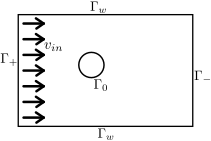
\includegraphics[width=0.7\textwidth]{domain_vector_2}
        \caption{The flow domain. The fluid flows in from the left and flows out on the right. There is no fluid flow through the top and bottom.}
        \label{flow_domain}
    \end{figure}
    
    The Navier-Stokes equations are non-linear therefore they have to be solved iteratively. Newton's method is used which in general gives increasingly good approximations to the solution of the equation $F(x_{sol}) = 0$ by solving $F(x_{cur}) + \delta F(x_{cur}, \delta x) = 0$ until  $F(x_{cur})$ is smaller than the tolerance limit. $\delta F$ is $F$ expanded to first order changes and it is linear in $\delta x$. After every iteration $x_{cur}$ is updated as $x_{new} = x_{old} + \delta x$. If $x_{cur}$ satisfies the boundary conditions and if $\delta x$ satisfies the homogeneous boundary conditions than after every iteration the solution will satisfy the boundary conditions.
    
    In the current case the linearised equation is to be solved for $(\mathbf{w}, r)$:
    \begin{equation}
    F(\mathbf{u_0}, p_0) + \delta F((\mathbf{u_0}, p_0), (\mathbf{w}, r)) = 0
    \end{equation}
    where
    \begin{equation}
    F(\mathbf{u_0}, p_0) =
    \begin{pmatrix}
    \rho \, (\mathbf{u_0 \cdot} \boldsymbol{\nabla}) \mathbf{u_0} + 
    \boldsymbol{\nabla} p_0 - 
    \mu \nabla^2 \mathbf{u_0} \\
    \boldsymbol{\nabla} \mathbf{\cdot u_0}
    \end{pmatrix}
    \end{equation}
    and
    \begin{equation}
    \delta F((\mathbf{u_0}, p_0), (\mathbf{w}, r)) = 
    \begin{pmatrix}
    \rho \, (\mathbf{w \cdot} \boldsymbol{\nabla}) \mathbf{u_0} + 
    \rho \, (\mathbf{u_0 \cdot} \boldsymbol{\nabla}) \mathbf{w} + 
    \boldsymbol{\nabla} r - 
    \mu \nabla^2 \mathbf{w} \\
    \boldsymbol{\nabla} \mathbf{\cdot w}
    \end{pmatrix}
    \end{equation}
    where $(\mathbf{u_0}, p)$ satisfies the boundary conditions of the flow (equation~\ref{flow_boundary_conditions}) and $(\mathbf{w}, r)$ satisfies the homogeneous boundary conditions:
    \begin{equation} \label{homogeneous_flow_boundary_conditions}
    \begin{cases}
    \mathbf{w} = 0 & \text{on } \Gamma_+ \\
    \frac{\partial w_x}{\partial n} = 0 & \text{on } \Gamma_w \\
    w_y = 0  & \text{on } \Gamma_w \\
    r \, \mathbf{n} - \mu \frac{\partial \mathbf{w}}{\partial n} = 0 & \text{on } \Gamma_- \\
    \mathbf{w} = 0 & \text{on } \Gamma_0
    \end{cases}
    \end{equation}
    
    The initial guess for the solution is the solution of the steady Stokes flow which is described by the following (linear) equations:
    \begin{equation} \label{Stokes_1}
    0 =\boldsymbol{\nabla} p - \mu \nabla^2 \mathbf{u}
    \end{equation}
    \begin{equation} \label{Stokes_2}
    0 = \boldsymbol{\nabla} \mathbf{\cdot u}
    \end{equation}
    where $(\mathbf{u}, p)$ satisfies the boundary conditions of the flow (equation~\ref{flow_boundary_conditions}). This is the limiting solution in the case of small Reynolds numbers where $Re = v \, D \, \rho \, / \, \mu$.
    
    \subsection{Force on the airfoil}
    For a flow the stress tensor is:
    \begin{equation} \label{stress_tensor}
    T_{ij} = -p \, \delta_{ij} +
    \mu \, \bigg{(}\frac{\partial u_i}{\partial x_j} + \frac{\partial u_j}{\partial x_i} \bigg{)}
    \end{equation}
    The drag force on the airfoil in a given direction $\mathbf{\hat{a}}$ is the opposite of the force on the fluid and is given by:
    \begin{equation} \label{direct_force}
    \mathcal{J} = \int\limits_{\Gamma_0} -a_i T_{ij} n_j \, \mathrm{d}s
    \end{equation}
    where summation convention was used and $\mathbf{\hat{n}}$ is the unit vector pointing out of the domain. If we introduce the smoothing function $\phi$ which is $0$ on the outer boundaries and $1$ on the inside boundary we can write the drag force as:
    \begin{equation} \label{direct_force_phi}
    \mathcal{J} = \int\limits_{\partial \Omega} - \phi \, a_i T_{ij} n_j \, \mathrm{d}s
    \end{equation}
    where
    \begin{equation} \label{phi_definition}
    \nabla^2 \phi = 0 \quad \text{inside}\ \Omega
    \qquad \text{and} \qquad
    \phi = \begin{cases}
    0	 &	\text{on}\ \Gamma_+, \Gamma_w, \Gamma_- \\
    1	 &	\text{on}\ \Gamma_0
    \end{cases}
    \end{equation}
    
    Then using the divergence theorem this can be written as:
    \begin{equation} \label{force_divergence}
    \mathcal{J} = \int\limits_{\Omega} - \frac{\partial}{\partial x_j}\big{(}\phi \, a_i T_{ij} \big{)} \, \mathrm{d}x
    \end{equation}
    which gives our cost function after expansion:
    \begin{equation} \label{cost_function}
    \mathcal{J} = \int\limits_{\Omega}{{p\, \mathbf{a \cdot} \boldsymbol{\nabla} \phi} -
        {\mu \boldsymbol{\nabla}(\mathbf{a \cdot u}) \mathbf{\cdot} \boldsymbol{\nabla} \phi} - 
        {\mu a_i \frac{\partial u_j}{\partial x_i} \frac{\partial \phi}{\partial x_j}} - 
        {\rho \phi \, \mathbf{u \cdot} \boldsymbol{\nabla}(\mathbf{a \cdot u})}
        \,  \mathrm{d}x}
    \end{equation}
    where the Navier-Stokes equations (\ref{NS_1} and \ref{NS_2}) were used.
    
    \subsection{Changing the domain}
    When we change the shape of the airfoil (so the domain) the flow will also change. The deformation of the domain can be described with the domain deformation vector field $\mathbf{V}$ which gives the position derivative at each point. If some point is at position $\mathbf{r_0}$ if some parameter has value $p_0$ then (in first order) the position of that point will be $\mathbf{r_0} + \epsilon \mathbf{V}$ if the parameter is changed to $p_0 + \epsilon$.
    
    As the flow always satisfies the Navier-Stokes equations (equations \ref{NS_1} and \ref{NS_2}) the derivative of the flow $(\mathbf{u'}, p')$ satisfies the Navier-Stokes equations expanded to first order changes:
    \begin{equation} \label{NS_der_1}
    0 = \rho (\mathbf{u' \cdot} \boldsymbol{\nabla}) \mathbf{u} + 
    \rho (\mathbf{u \cdot} \boldsymbol{\nabla}) \mathbf{u'} + 
    \boldsymbol{\nabla} p' - 
    \mu \nabla^2 \mathbf{u'}
    \end{equation}
    \begin{equation} \label{NS_der_2}
    0 = \boldsymbol{\nabla} \mathbf{\cdot u'}
    \end{equation}
    
    On non-deformed boundaries the boundary conditions for a function's derivative ($f'$) come from expanding the boundary conditions of $f$ to first order changes. On deformed boundaries with Dirichlet boundary conditions of constant value the original boundary conditions should be expanded to first order changes:
    \begin{equation}
    f(\mathbf{x}) = (f + \epsilon f') (\mathbf{x} + \epsilon \mathbf{V}) =
    f(\mathbf{x}) + \epsilon f'(\mathbf{x}) + \epsilon \mathbf{V \cdot} \boldsymbol{\nabla} f
    \end{equation}
    \begin{equation}
    f' = - \mathbf{V \cdot} \boldsymbol{\nabla} f
    \end{equation}
    where $\mathbf{V}$ is the domain deformation vector. This simplifies due to the Dirichlet boundary condition:
    \begin{equation}
    f' = - \mathbf{V \cdot} \boldsymbol{\nabla} f = 
    - \frac{\partial f}{\partial n} (\mathbf{V \cdot n}) -
    \frac{\partial f}{\partial \tau_j} (\mathbf{V \cdot} \boldsymbol{\tau}_j) = 
    - \frac{\partial f}{\partial n} (\mathbf{V \cdot n})
    \end{equation}
    See also Lemma 2.2 in Schmidt and Schultz's paper \cite{Schmidt_1}. The boundary conditions therefore for the derivatives $(\mathbf{u'}, p')$ and $\phi'$ are:
    \begin{equation} \label{flow_der_boundary_conditions}
    \begin{cases}
    \mathbf{u'} = 0 & \text{on } \Gamma_+ \\
    \frac{\partial u'_x}{\partial n} = 0 & \text{on } \Gamma_w \\
    u'_y = 0  & \text{on } \Gamma_w \\
    p' \, \mathbf{n} - \mu \frac{\partial \mathbf{u'}}{\partial n} = 0 & \text{on } \Gamma_- \\
    \mathbf{u'} = - (\mathbf{V \cdot n}) \frac{\partial \mathbf{u}}{\partial n} & \text{on } \Gamma_0
    \end{cases}
    \end{equation}
    and
    \begin{equation} \label{phi_der_boundary_conditons}
    \phi' = \begin{cases}
    0	 &	\text{on}\ \Gamma_+, \Gamma_w, \Gamma_- \\
    - (\mathbf{V \cdot n}) \frac{\partial \phi}{\partial n}	 &	\text{on}\ \Gamma_0
    \end{cases}
    \end{equation}
    
    \subsection{Derivative of the force}
    The change in the cost function arises from the change in the domain and the change in the flow. Using adjoint states the derivative of the force of the airfoil is given by:
    \begin{equation} \label{cost_derivative_definition}
    \begin{split}
    d \mathcal{J} = \int\limits_{\Gamma_0}(\mathbf{V \cdot n}) \, \bigg{(} &
    \mu \boldsymbol{\nabla}(\mathbf{a \cdot u}) \mathbf{\cdot} \boldsymbol{\nabla} \phi -
    \mu \frac{\partial u_i}{\partial x_j} \frac{\partial w_i}{\partial x_j}
    \bigg{)} \, \mathrm{d}s
    \end{split}
    \end{equation}
    with adjoint state $(\mathbf{w},r)$. Note that the variables $(\mathbf{w},r)$ are re-used and this adjoint state does not equal to the state calculated upon solving the Navier-Stokes equations. It is described by the equations:
    \begin{equation} \label{adj_velocity_definition}
    \begin{split}
    0 = & -\rho w_j \frac{\partial u_j}{\partial x_i} +
    \rho (\mathbf{u \cdot} \boldsymbol{\nabla}) w_i +
    \mu \nabla^2 w_i +
    \frac{\partial r}{\partial x_i} \\ 
    & -\mu \frac{\partial (\mathbf{a \cdot} \boldsymbol{\nabla} \phi)}{\partial x_i} +
    \rho \phi \frac{\partial (\mathbf{a \cdot u})}{\partial x_i} - 
    \rho a_i (\mathbf{u \cdot} \boldsymbol{\nabla} \phi)
    \end{split}
    \end{equation}
    \begin{equation} \label{adj_pressure_definition}
    0 = \boldsymbol{\nabla} \mathbf{\cdot w} - 
    \mathbf{a \cdot} \boldsymbol{\nabla} \phi
    \end{equation}
    The boundary conditions are:
    \begin{equation}
    \begin{cases}
    \mathbf{w} = 0	 	&	\text{on}\ \Gamma_+ \\
    \frac{\partial w_x}{\partial n} - a_x (\boldsymbol{\nabla} \phi \mathbf{\cdot n}) - 
    \frac{\partial \phi}{\partial x} (\mathbf{a \cdot n}) = 0	&	\text{on}\ \Gamma_w \\
    w_y = 0				&	\text{on}\ \Gamma_w \\
    r \, \mathbf{n} + \mu \frac{\partial \mathbf{w}}{\partial n} + \rho \, \mathbf{w} (\mathbf{u \cdot n}) - 
    \mu \, \mathbf{a} (\boldsymbol{\nabla} \phi \mathbf{\cdot n}) - 
    \mu \boldsymbol{\nabla} \phi (\mathbf{a \cdot n}) = 0	   	&	\text{on}\ \Gamma_- \\
    \mathbf{w} = 0	 	&	\text{on}\ \Gamma_0
    \end{cases}
    \end{equation}
    For the full derivation see Appendix~\ref{app:force}. It can be seen that the differential equations have to be solved only once and then for any shape change (for any $\mathbf{V}$) the cost function derivative is given by a surface integral of $(\mathbf{V \cdot n}) \, f$ for some function $f$. If the deformation is set to $\mathbf{V} \propto f\, \mathbf{n}$ then the shape can be optimised without the need of any parametrisation. 
    
    \subsection{Stability of the flow}
    For a steady base flow $(\mathbf{u},p)$ if we perturb the flow field the state equations of the perturbation field $(\mathbf{w},r)$ are the Navier-Stokes equations expanded to first order changes.
    \begin{equation}
    0 = \rho \, \mathbf{\dot{w}} + 
    \rho \, (\mathbf{w \cdot} \boldsymbol{\nabla}) \mathbf{u} + 
    \rho \, (\mathbf{u \cdot} \boldsymbol{\nabla}) \mathbf{w} + 
    \boldsymbol{\nabla} r - 
    \mu \, \nabla^2 \mathbf{w}
    \end{equation}
    \begin{equation}
    0 = \boldsymbol{\nabla} \mathbf{\cdot w}
    \end{equation}
    Note that the variables $(\mathbf{w}, r)$ are re-used again and the perturbation state does not equal to the adjoint state used when the derivative of the force was calculated. When we are searching for normal modes the perturbation field should be in the form $(\mathbf{w}(t),r(t) = (\mathbf{w},r) \, e^{st})$ where both $(\mathbf{w},r)$ and $s$ are complex. The real part of $s$ is the exponential growth of the amplitude and the imaginary part is the angular frequency of the oscillations. If the perturbation field has this form the state equations become:
    \begin{equation} \label{perturbation_1}
    \rho \, (\mathbf{w \cdot} \boldsymbol{\nabla}) \mathbf{u} + 
    \rho \, (\mathbf{u \cdot} \boldsymbol{\nabla}) \mathbf{w} + 
    \boldsymbol{\nabla} r - 
    \mu \, \nabla^2 \mathbf{w} = 
    - \rho \, s \, \mathbf{w} 
    \end{equation}
    \begin{equation} \label{perturbation_2}
    \boldsymbol{\nabla} \mathbf{\cdot w} = 0
    \end{equation}
    The boundary conditions are:
    \begin{equation} \label{perturbation_bcs}
    \begin{cases}
    \mathbf{w} = 0 & \text{on } \Gamma_+ \\
    \frac{\partial w_x}{\partial n} = 0 & \text{on } \Gamma_w \\
    w_y = 0 & \text{on } \Gamma_w \\
    r \, \mathbf{n} - \mu \frac{\partial \mathbf{w}}{\partial n} = 0 & \text{on } \Gamma_- \\
    \mathbf{w} = 0 & \text{on } \Gamma_0 \\
    \end{cases}
    \end{equation}
    This is an eigenvalue equation for $(\mathbf{w},r)$ which has multiple solutions. Usually the most unstable mode which is the one with the highest real part is the most influential. The field is fixed only up to an arbitrary complex multiplicative factor. As the left hand side of eigenvalue equation is purely real if $s$ is an eigenvalue then its complex conjugate $s^*$ is also an eigenvalue.
    
    \subsection{Derivative of the eigenvalue}
    If we change the domain, the derivative of the perturbation field is given by:
    \begin{equation} \label{perturbation_change_1}
    \begin{split}
    0 = \ & \rho \, s' \, \mathbf{w} + 
    \rho \, s \, \mathbf{w'} + 
    \rho \, (\mathbf{w \cdot} \boldsymbol{\nabla}) \mathbf{u'} + 
    \rho \, (\mathbf{w' \cdot} \boldsymbol{\nabla}) \mathbf{u} \ + \\
    &\rho \, (\mathbf{u' \cdot} \boldsymbol{\nabla}) \mathbf{w} + 
    \rho \, (\mathbf{u \cdot} \boldsymbol{\nabla}) \mathbf{w'} +
    \boldsymbol{\nabla} r' - 
    \mu \, \nabla^2 \mathbf{w'}
    \end{split}
    \end{equation}
    \begin{equation} \label{perturbation_change_2}
    0 = \boldsymbol{\nabla} \mathbf{\cdot w'}
    \end{equation}
    The boundary conditions are:
    \begin{equation} \label{perturbation_change_bcs}
    \begin{cases}
    \mathbf{w'} = 0 & \text{on } \Gamma_+ \\
    \frac{\partial w'_x}{\partial n} = 0 & \text{on } \Gamma_w \\
    w'_y = 0 & \text{on } \Gamma_w \\
    r' \, \mathbf{n} - \mu \frac{\partial \mathbf{w'}}{\partial n} = 0 & \text{on } \Gamma_- \\
    \mathbf{w'} = - (\mathbf{V \cdot n}) \frac{\partial \mathbf{w}}{\partial n} & \text{on } \Gamma_0 \\
    \end{cases}
    \end{equation}
    
    The cost function to be investigated now is the eigenvalue of a perturbation state $(\mathbf{w}, r)$.
    \begin{equation} \label{cost_function_eigenvalue}
    \mathcal{J} = s
    \end{equation}
    
    The derivative of the cost function is given by:
    \begin{equation}
    d \mathcal{J} = s' = \int\limits_{\Gamma_0} - (\mathbf{V \cdot n}) \left( 
    \mu \, \frac{\partial u_i}{\partial x_j} \frac{\partial u^{\dagger*}_i}{\partial x_j} + 
    \mu \, \frac{\partial w_i}{\partial x_j} \frac{\partial w^{\dagger*}_i}{\partial x_j}
    \right) \, \mathrm{d} s 
    \end{equation}
    where $(\mathbf{w},r)$ is the normalised perturbation field, $(\mathbf{u^{\dagger*}},p^{\dagger*})$ is the complex conjugate of the adjoint base flow and $(\mathbf{w^{\dagger*}},r^{\dagger*})$ is the complex conjugate of the adjoint perturbation field. Note that the adjoint perturbation field is not the perturbation field of the adjoint base flow.
    
    The equations of the complex conjugate of the adjoint perturbation field $(\mathbf{w^{\dagger*}},r^{\dagger*})$ are:
    \begin{equation}
    \rho \, \mathbf{w^{\dagger*} \cdot} \frac{\partial \mathbf{u}}{\partial x_i} - 
    \rho \, (\mathbf{u \cdot} \boldsymbol{\nabla}) w^{\dagger*}_i - 
    \mu \, \nabla^2 w^{\dagger*}_i - 
    \frac{\partial r^{\dagger*}}{\partial x_i} = 
    -\rho \, s \, w^{\dagger*}_i
    \end{equation}
    \begin{equation}
    \boldsymbol{\nabla} \mathbf{\cdot w^{\dagger*}} = 0
    \end{equation}
    with boundary conditions:
    \begin{equation}
    \begin{cases}
    \mathbf{w^{\dagger*}} = 0 & \text{on } \Gamma_+ \\
    \frac{\partial w^{\dagger*}_x}{\partial n} = 0 & \text{on } \Gamma_w \\
    w^{\dagger*}_y = 0 & \text{on } \Gamma_w \\
    \rho \, \mathbf{w^{\dagger*}} (\mathbf{u \cdot n}) + \mu \, \frac{\partial \mathbf{w^{\dagger*}}}{\partial n} + 
    r^{\dagger*} \, \mathbf{n} = 0 & \text{on } \Gamma_- \\
    \mathbf{w^{\dagger*}} = 0 & \text{on } \Gamma_0
    \end{cases}
    \end{equation}
    Since these equations are homogeneous and linear in $(\mathbf{w^{\dagger*}}, r^{\dagger*})$ the zero state is a trivial solution. To find the actual (non-trivial) solution one needs to find solutions of the eigenvalue equation (as if $s$ were free to vary) and choose the solution from the found eigenvalues which is closest to the eigenvalue found during the stability analysis. The difference between the two eigenvalues should be due to computational errors.
    
    The perturbation state $(\mathbf{w}, r)$ needs to be normalised using the constraint:
    \begin{equation}
    0 = 1 + \int\limits_{\Omega}
    \rho \, (\mathbf{w^{\dagger*} \cdot w})
    \, \mathrm{d} x
    \end{equation}
    The purpose of this is to ensure that all the volume terms vanish in the expression of the derivative of the eigenvalue.
    
    The equations of the adjoint base flow's complex conjugate $(\mathbf{u^{\dagger*}}, p^{\dagger*})$ are:
    \begin{equation}
    0 = - \rho \, (\mathbf{u \cdot} \boldsymbol{\nabla}) u^{\dagger*}_i + 
    \rho \, \mathbf{u^{\dagger*} \cdot} \frac{\partial \mathbf{u}}{\partial x_i} - 
    \mu \, \nabla^2 u^{\dagger*}_i - 
    \frac{p^{\dagger*}}{\partial x_i} + 
    \rho \, \mathbf{w^{\dagger*} \cdot} \frac{\partial \mathbf{w}}{\partial x_i} - 
    \rho \, (\mathbf{w \cdot} \boldsymbol{\nabla}) w^{\dagger*}_i
    \end{equation}
    \begin{equation}
    0 = \boldsymbol{\nabla} \mathbf{\cdot u^{\dagger*}}
    \end{equation}
    with boundary conditions
    \begin{equation}
    \begin{cases}
    \mathbf{u^{\dagger*}} = 0 & \text{on } \Gamma_+ \\
    \frac{\partial u^{\dagger*}_x}{\partial n} = 0 & \text{on } \Gamma_w \\
    u^{\dagger*}_y = 0 & \text{on } \Gamma_w \\
    \rho \, \mathbf{u^{\dagger*}} (\mathbf{u \cdot n}) + \mu \, \frac{\partial \mathbf{u^{\dagger*}}}{\partial n} + 
    p^{\dagger*} \, \mathbf{n} + \rho \, \mathbf{w^{\dagger*}} (\mathbf{w \cdot n}) = 0 & \text{on } \Gamma_- \\
    \mathbf{u^{\dagger*}} = 0 & \text{on } \Gamma_0
    \end{cases}
    \end{equation}
    For the full derivation see Appendix~\ref{app:eigenvalue}.
    
\section{Results and discussion}
\subsection{General properties of the program}
The differential equations are solved an open source finite element package called Fenics (fenicsproject.org). It is capable of solving linear differential equations as well as eigenvalue equations using the SLEPc package.

\subsubsection{Weak form of equations}
Fenics can only solve a differential equation if it is put into the weak form. This means that the equation needs to be multiplied by a test function $(\mathbf{v}, q)$ and integrated over the domain. Then for any test function with the same number of degrees of freedom the equation needs to be true. Also the terms in the equation with the highest derivatives need to be integrated partially until the degree of the highest derivative of the test function is the same as the degree of the highest derivative of the function to be solved (the trial function). If this is not possible one needs to ensure that the difference in the degrees is one. The Neumann or Robin boundary conditions are enforced during this step.

To take an example consider the equations of the Stokes flow. If they are multiplied with the test function $(\mathbf{v}, q)$ and integrated throughout the domain we get:
\begin{equation}
0 = \int\limits_{\Omega}
\mathbf{v \cdot} \left(
\boldsymbol{\nabla} p - \mu \nabla^2 \mathbf{u}
\right) +
q \boldsymbol{\nabla} \mathbf{\cdot u}
\, \mathrm{d}x
\end{equation}
If we integrate the first two terms by parts we get:
\begin{equation}
\begin{split}
0 = &\int\limits_{\Omega}
- \boldsymbol{\nabla} \mathbf{\cdot v} \, p  +
\mu \frac{\partial v_i}{\partial x_j} \frac{\partial u_i}{\partial x_j} +
q \boldsymbol{\nabla} \mathbf{\cdot u}
\, \mathrm{d}x \ + \\
&\int\limits_{\partial \Omega}
\mathbf{v \cdot n} \, p - 
\mu v_i \frac{\partial u_i}{\partial x_j} n_j
\, \mathrm{d}s
\end{split}
\end{equation}
The test function is zero where Dirichlet boundary conditions are specified and on other boundaries the integrand is zero due to the boundary conditions. This means that the boundary term is zero and the weak form is:
\begin{equation}
0 = \int\limits_{\Omega}
- \boldsymbol{\nabla} \mathbf{\cdot v} \, p  +
\mu \frac{\partial v_i}{\partial x_j} \frac{\partial u_i}{\partial x_j} +
q \boldsymbol{\nabla} \mathbf{\cdot u}
\, \mathrm{d}x
\end{equation}

\subsubsection{Mesh}
The program gmsh can be used to generate the mesh. The density of vertices is largest near the airfoil and decreases towards the outer boundaries. A mesh can be characterised by its 'resolution', meaning the number of vertices on the airfoil. The airfoil is enclosed by three bounding boxes. On Figure \ref{fig_mesh_full} a typical (lower resolution) mesh can be seen. The mesh closer to the airfoil is on Figure \ref{fig_mesh_close}. The mesh close to the leading and trailing edges at different resolutions can be seen on Figure \ref{fig_mesh_edges}. It can be seen that increasing resolution results not only in finer mesh but also smoother airfoils. It is important to have a large enough bounding box to capture the wake fully.
\begin{figure}[htbp]
    \centering
    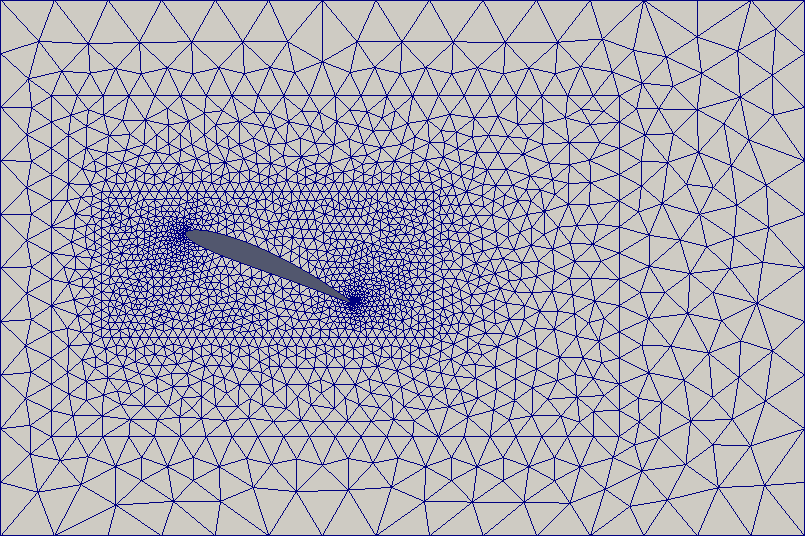
\includegraphics[height=5cm]{mesh_1}
    \caption{A typical mesh around the airfoil. A Joukowsky-like airfoil is surrounded by three bounding boxes. As the distance from the airfoil increases the mesh becomes coarser. In this case there are 50 vertices on the airfoil.}
    \label{fig_mesh_full}
\end{figure}
\begin{figure}[htbp]
    \centering
    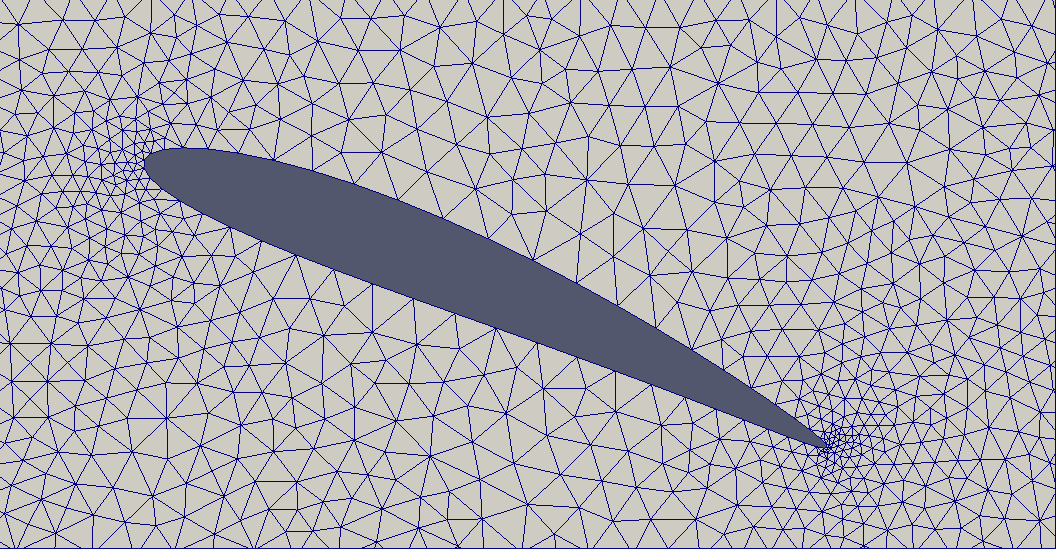
\includegraphics[height=5cm]{mesh_2}
    \caption{The mesh close to the airfoil. There are 50 vertices around a Joukowsky-like airfoil.}
    \label{fig_mesh_close}
\end{figure}
\begin{figure}[htbp]
    \centering
    \subfloat[][resolution = 50 \\
    leading edge]{
        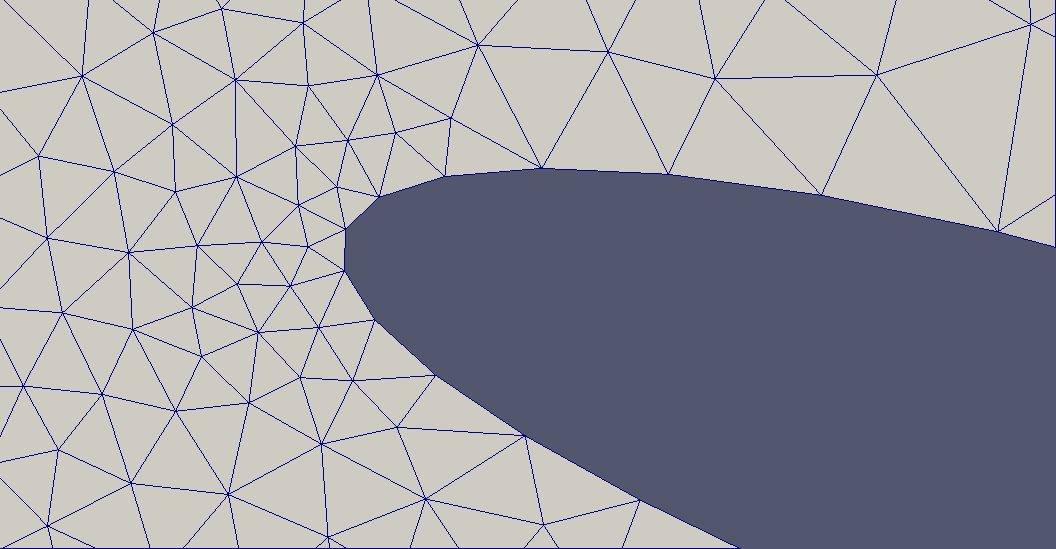
\includegraphics[width= 0.4\textwidth]{mesh_3}
    } \qquad
    \subfloat[][resolution = 50 \\
    trailing edge]{
        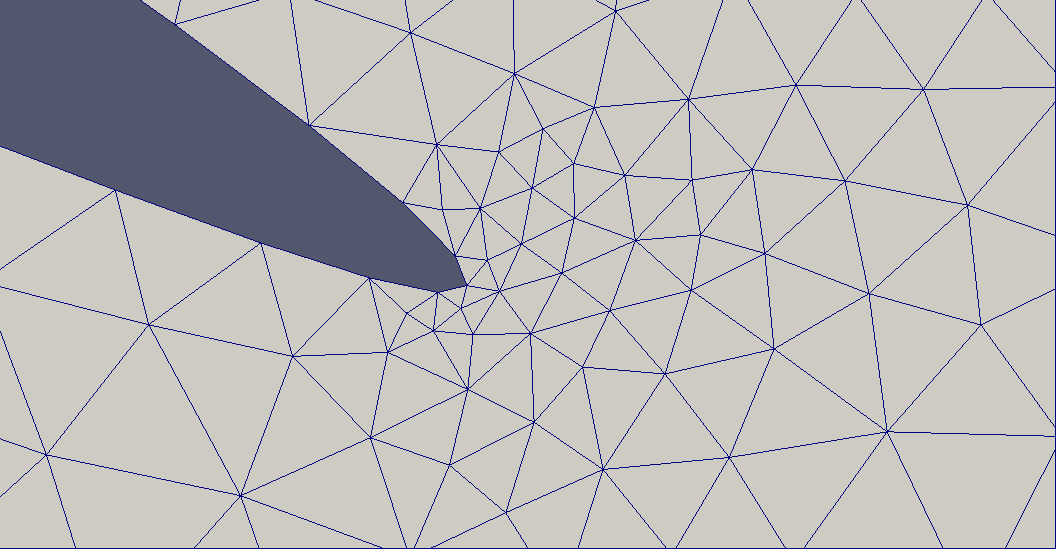
\includegraphics[width= 0.4\textwidth]{mesh_4}
    } \\
    \subfloat[][resolution = 250 \\
    leading edge]{
        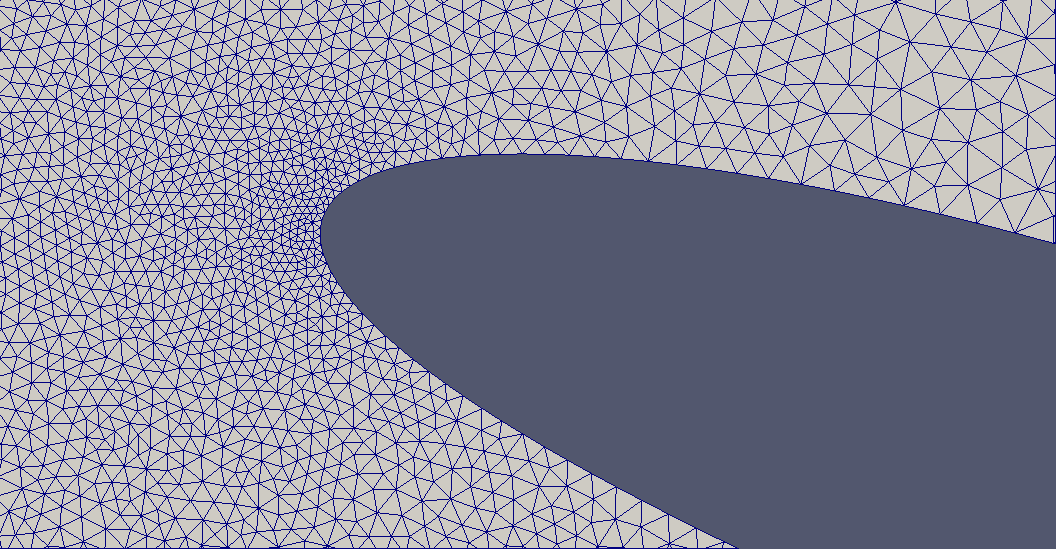
\includegraphics[width= 0.4\textwidth]{mesh_5}
    } \qquad
    \subfloat[][resolution = 250 \\
    trailing edge]{
        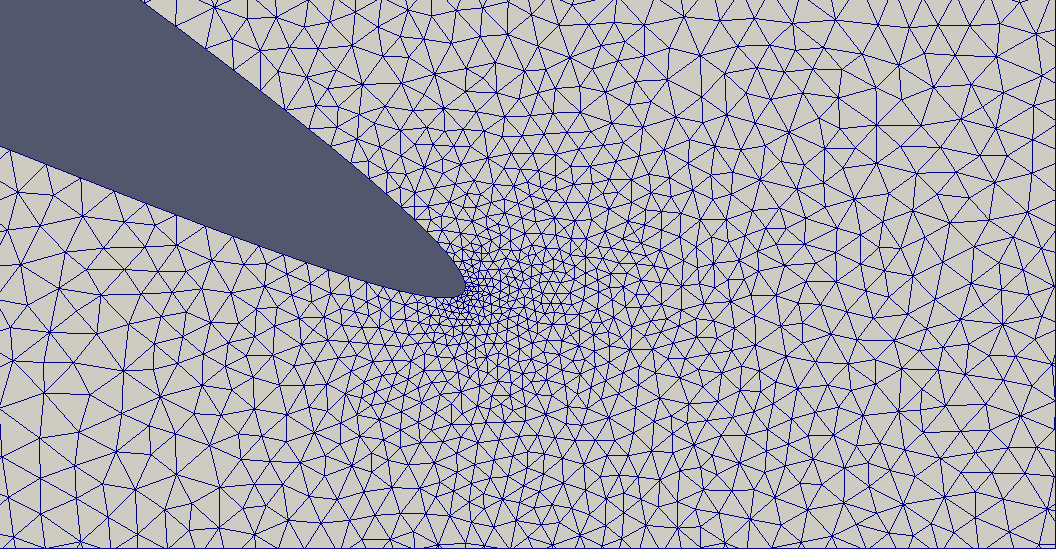
\includegraphics[width= 0.4\textwidth]{mesh_6}
    }
    \caption{Leading and trailing edges at two resolutions. It can be seen that at higher resolutions the mesh is finer and the airfoil surface is approximated more smoothly as well.}
    \label{fig_mesh_edges}
\end{figure}

\subsection{Flow around a cylinder}
The flow solver and the adjoint derivative was validated using a simple geometry. The flow around a circle cannot be calculated analytically but it can be compared with literature results. The calculated derivative can be compared with the numerical derivative of the force. The parameters of the flow were:
\begin{equation}
\begin{cases}
v_{in} = 1.0 \\
\rho = 1.0 \\
\mu = 0.5 \\
r_{circle} = 1.0
\end{cases}
\end{equation}
This gives a Reynolds number of $Re = 4.0$.

The pressure and velocity fields can be seen on Figure \ref{fig_circle}.
\begin{figure}[htbp]
    \centering
    \subfloat[][pressure]{
        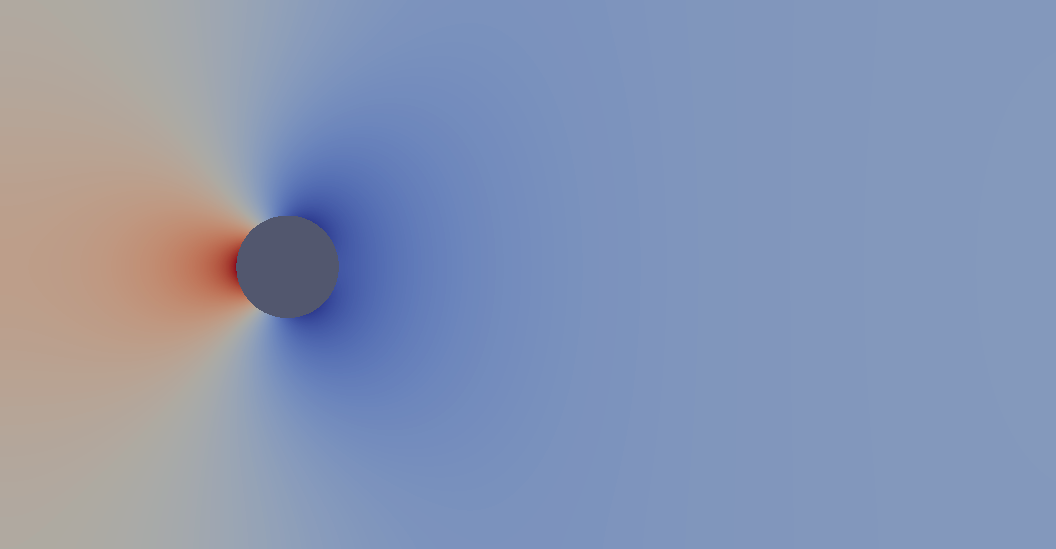
\includegraphics[width= 0.9\textwidth]{pressure_circle}
    } \\
    \subfloat[][velocity]{
        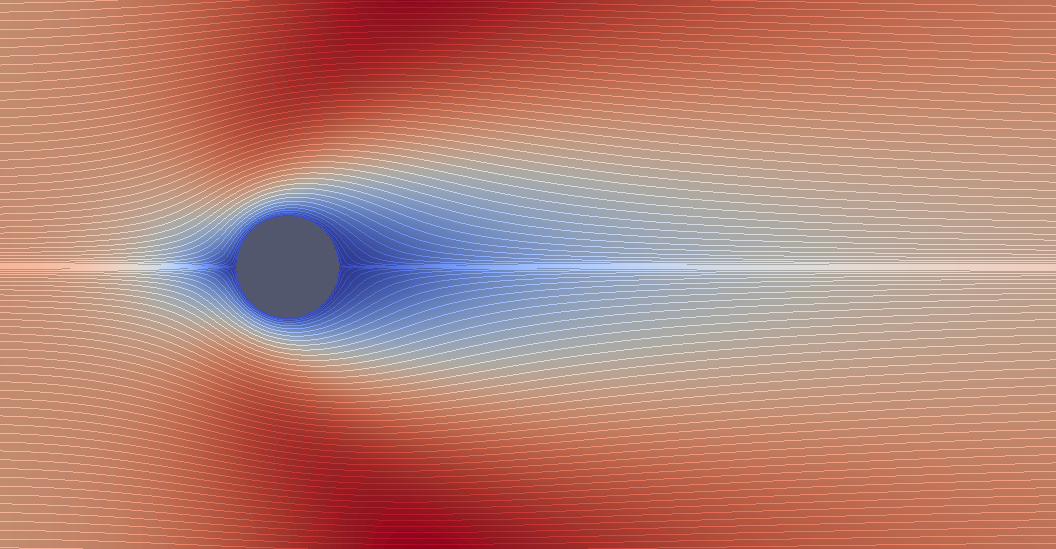
\includegraphics[width= 0.9\textwidth]{velocity_circle}
    }
    \caption{The pressure and velocity fields around a circle. The colour denotes the magnitude of the fields.}
    \label{fig_circle}
\end{figure}

The drag force calculated using Gauss's theorem was compared with the drag force calculated using a surface integral on $\Gamma_0$ at multiple resolutions. The calculated force values and their difference as a functions of resolution can be seen on Figure~\ref{fig:circle_convergence}.

The two values showed good agreement with the difference becoming smaller as the resolution was increased. The method which uses Gauss's theorem converges faster than the direct calculation. THIS MIGHT BE BECAUSE .......

The drag force was $F_{drag} = 7.36$ which gives the (2D) drag coefficient:
%$F_{drag} = 7.36$.
%$C_d = 7.36$.
\begin{equation}
C_d = \frac{F_{\text{drag}}}{\frac{1}{2} \rho v^2 d} = 7.36
\end{equation}
\begin{figure}[hbtp]
    \centering
    \subfloat[]{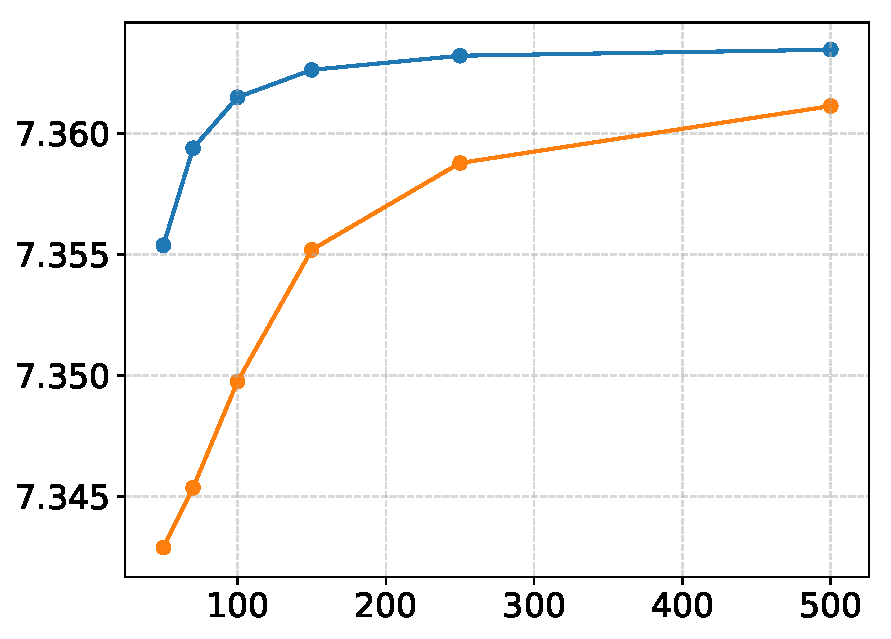
\includegraphics[width=0.4\textwidth]{circ_force_val_conv_plot}}
    \qquad
    \subfloat[]{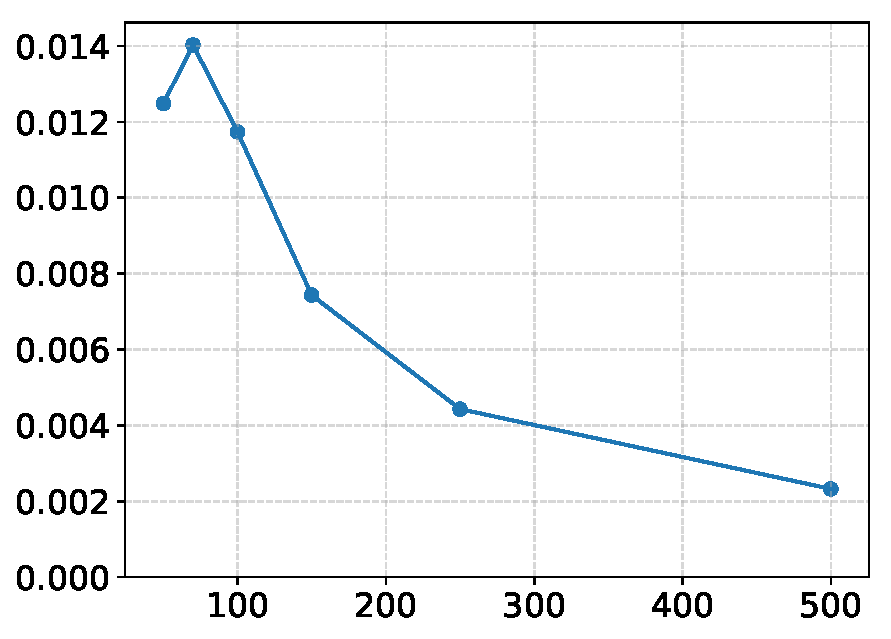
\includegraphics[width=0.4\textwidth]{circ_force_diff_conv_plot}}
    \caption{INCLUDE AXIS TITLES+LEGEND! The convergence of two methods for calculating the drag force on a circle. On figure (a) the convergence of the calculated drag forces can be seen as a function of resolution. On figure (b) the difference between the two methods can be seen as a function of resolution. INCLUDE AXIS TITLES+LEGEND!}
    \label{fig:circle_convergence}
\end{figure}

Using a circular geometry is beneficial because in the derivative of the drag force, $(\mathbf{V \cdot n}) = -1$ throughout the boundary $\Gamma_0$. This makes the calculations easier. The derivative of the drag force with respect to the radius of the airfoil was calculated using both the finite differences method and the adjont method discussed previously. They showed good agreement with the difference becoming smaller and smaller as the resolution was increased. The derivative of the drag force was $F'_{drag} = 6.36$ so the derivative of the drag coefficient is:
%$F'_{drag} = 6.36$.
%$C'_d = -1.00$
\begin{equation}
C'_d = -1.00
\end{equation}

\subsection{Flow around an ellipse}
The flow around an ellipse was also calculated. The ellipse was parametrised with the semi-major and semi-minor axes ($a$ and $b$) and the angle of rotation $\alpha$. The parameters of the flow were:
\begin{equation}
\begin{cases}
v_{in} = 1.0 \\
\rho = 1.0 \\
\mu = 0.5 \\
a = 1.2 \\
b = 0.8
\end{cases}
\end{equation}
and $\alpha$ was varied. The Lift-Drag ratio was maximised. The flow field around the optimised ellipse can be seen on Figure \ref{fig_opt_ellipse}. The angle between the horizontal and the longer axis is $41.84^{\circ}$. The Lift-Drag ratio is $0.135$. The angle of attack is large but no recirculation zones appear. This is probably because the Reynolds number is small and the shape is not very different from a circle.
\begin{figure}[htbp]
    \centering
    \subfloat[][pressure]{
        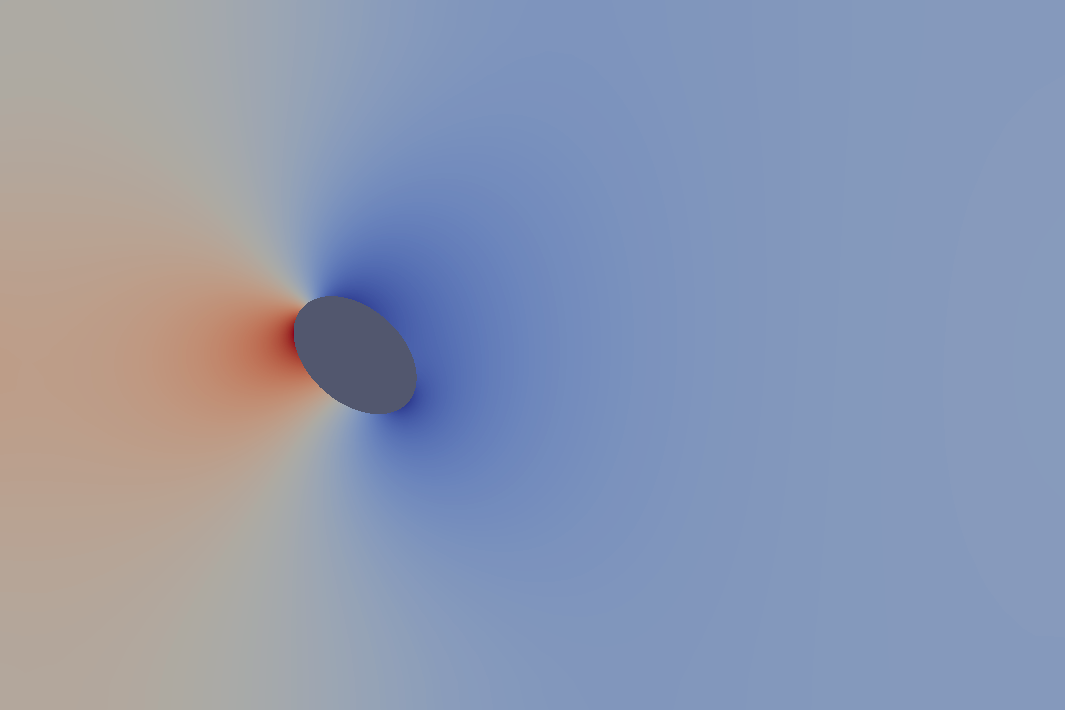
\includegraphics[width= 0.9\textwidth]{pressure_ellipse_opt}
    } \qquad
    \subfloat[][velocity]{
        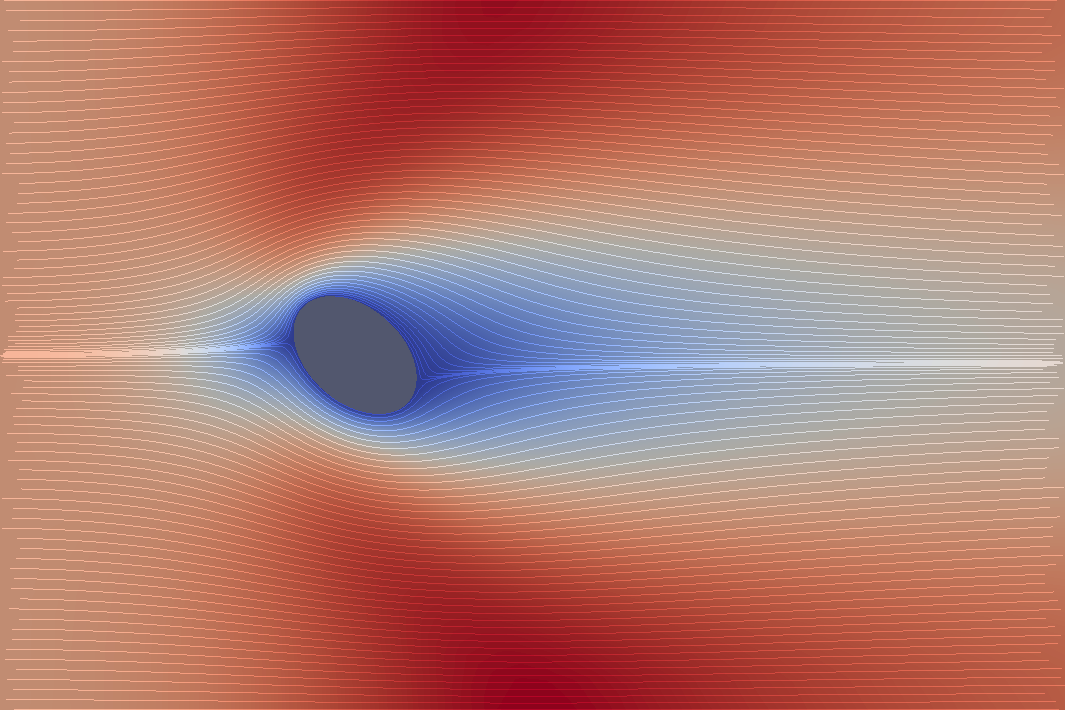
\includegraphics[width= 0.9\textwidth]{velocity_ellipse_opt}
    }
    \caption{The flow around an ellipse at optimal angle of attack. The colour denotes the magnitude of the fields. The angle between the horizontal and the longer axis of the ellipse is $41.84^{\circ}$. The Lift-Drag ratio is $0.135$.}
    \label{fig_opt_ellipse}
\end{figure}

\subsection{The shape of a Joukowsky-like airfoil}
A Joukowsky airfoil has one complex parameter $c$ and is described by the points on the complex plane $\zeta$:
\begin{equation}
\zeta = z + \frac{1}{z} \quad \text{where} \quad 
z = (1+c) \, e^{i \Theta} - c , \quad
0 \leq \Theta \leq 2 \pi
\end{equation}
This airfoil has a sharp trailing edge which is undesirable. Also it is beneficial if the airfoil can be rotated. Therefore the used Joukowsky-like airfoil is described by three parameters, the real and imaginary parts of $c$ and an angle of rotation $\alpha$ ($p = (\Re \lbrack c \rbrack, \Im \lbrack c \rbrack, \alpha)$ is a vector of parameters). The points on the airfoil are given by:
\begin{equation}
\zeta = \left( z + \frac{1}{z} \right) \, e^{i \alpha} \quad \text{where} \quad 
z = b + (1+c) \, e^{i \Theta} - c , \quad
0 \leq \Theta \leq 2 \pi
\end{equation}
The parameter $b$ is needed to avoid the sharp trailing edge and its value was chosen to be $b = -0.05$. Note that with this airfoil not every value of $\Re \lbrack c \rbrack$ is permitted. If it is too large then the airfoil becomes overlapping (similarly to an infinity sign $\infty$) so it needs to be ensured that $\Re \lbrack c \rbrack < -0.025$.

\subsection{Optimising the angle of the airfoil}
First only the angle was varied. The parameters of the flow were:
\begin{equation}
\begin{cases}
v_{in} = 1.0 \\
\rho = 1.0 \\
\mu = 0.1 \\
p = (-0.1,\, -0.05,\, \alpha)
\end{cases}
\end{equation}
The angle of attack was varied between $0^\circ$ and $90^\circ$. The measured Lift-Drag ratio can be seen on Figure \ref{fig_lift_drag}. it is first increasing up to approximately $25^\circ$ than it is decreasing. The curve is smooth because the Reynolds number is low so the steady state is stable for any angle of incidence. The peak of the curve occurs at $\alpha = (-) 23.78^\circ$ and the maximum value is $(L/D)_{max} = 1.154$. The pressure and velocity fields can be seen on Figure \ref{fig_opt_angle}.
\begin{figure}[htbp]
    \centering
    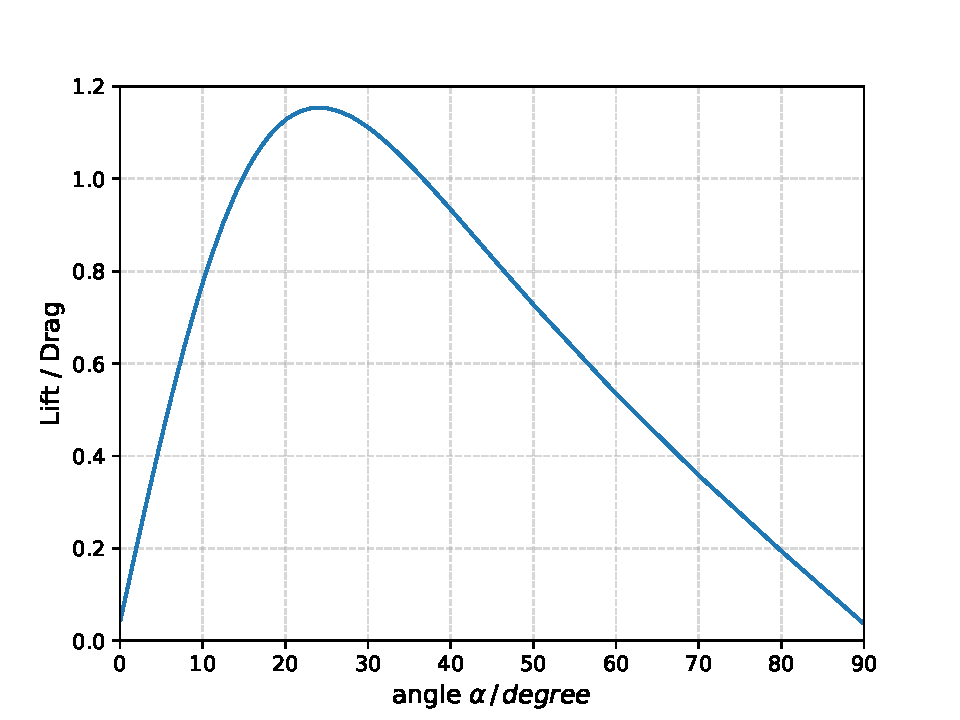
\includegraphics[height=5cm]{lift_drag.pdf}
    \caption{Lift/Drag as a function of angle. A resolution of 50 was used. The curve is smooth and it has a maximum at $\alpha = 23.78^\circ$.}
    \label{fig_lift_drag}
\end{figure}
\begin{figure}[htbp]
    \centering
    \subfloat[][pressure]{
        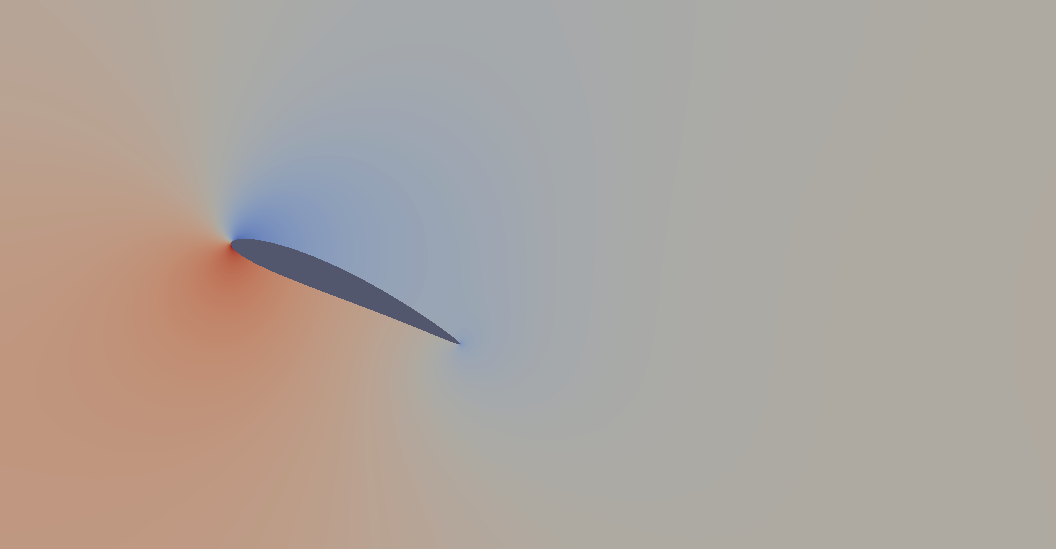
\includegraphics[width= 0.9\textwidth]{pressure_angle}
    } \\
    \subfloat[][velocity]{
        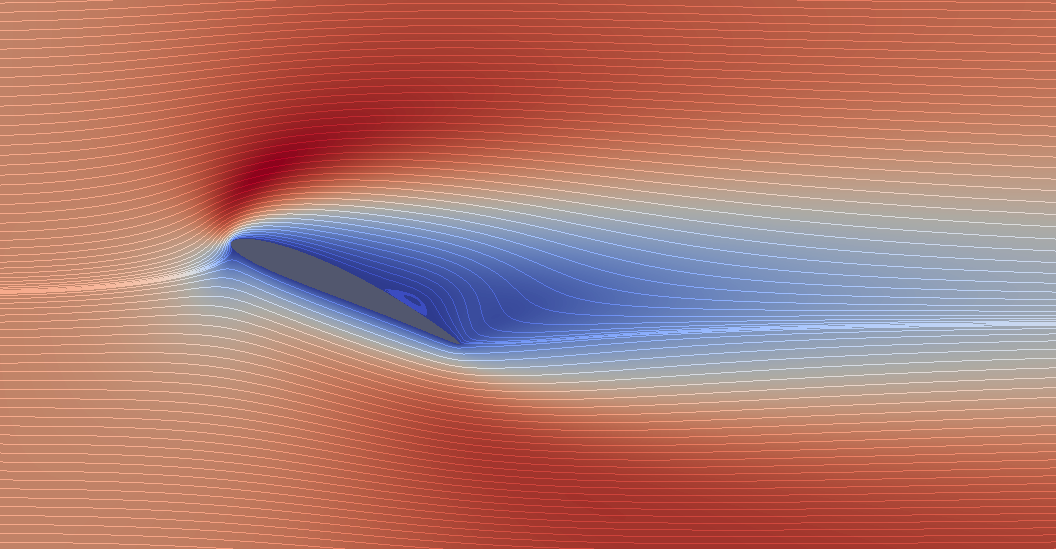
\includegraphics[width= 0.9\textwidth]{velocity_angle}
    }
    \caption{The pressure and velocity fields at optimal angle of attack. The colour denotes the magnitude of the fields. The angle of attack is $\alpha = 23.78^\circ$.}
    \label{fig_opt_angle}
\end{figure}

\subsection{Optimising the airfoil for Lift-Drag ratio}
Then the airfoil was searched with the highest possible Lift-Drag ratio. During the search the solution seemed to be in the region $\Re \lbrack c \rbrack > -0.025$ where the airfoil becomes overlapping. Therefore a 'repulsive' term was added to the cost function which keeps $\Re \lbrack c \rbrack < -0.025$ without the need of introducing a constraint and the cost function was:
\begin{equation}
\mathcal{J} = \frac{Lift}{Drag} + \frac{0.005}{\Re \lbrack c \rbrack + 0.025}
\end{equation}
and the derivative was
\begin{equation}
d \mathcal{J} = \frac{L'}{D} - \frac{D' \, L}{D^2} - \frac{0.005 \, d \Re \lbrack c \rbrack }{(\Re \lbrack c \rbrack + 0.025)^2}
\end{equation}
where $d \Re \lbrack c \rbrack$ is one if $\mathcal{J}$ is differentiated with respect to $\Re \lbrack c \rbrack$ and zero otherwise. This cost function does not maximise the Lift-Drag ratio but gives a reasonably good answer. The flow around the optimised airfoil can be seen on Figure \ref{fig_opt_joukow}. The optimal parameters were $p = (-0.0671,-0.2492,-0.4081)$.
\begin{figure}[htbp]
    \centering
    \subfloat[][pressure]{
        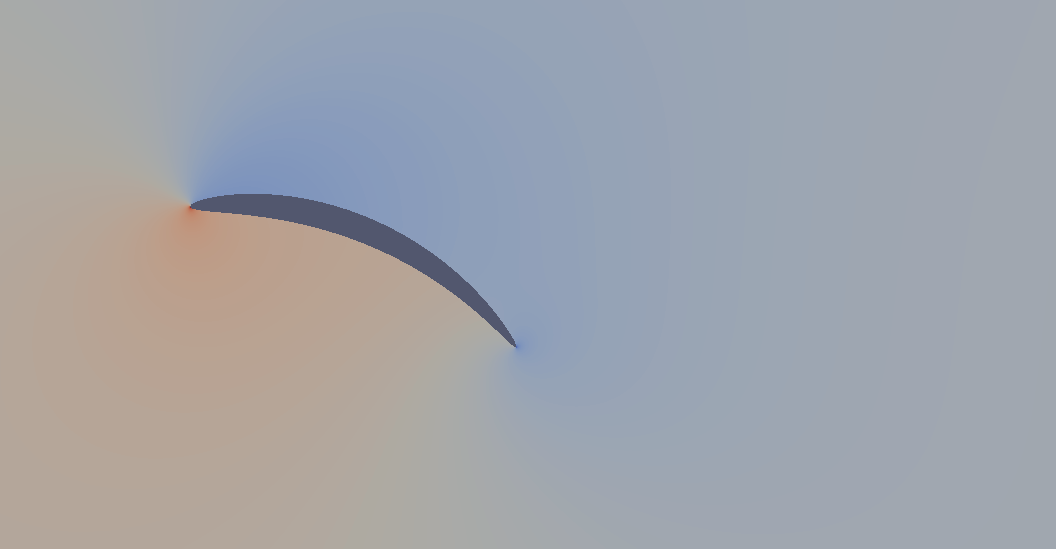
\includegraphics[width= 0.9\textwidth]{pressure_joukow}
    } \\
    \subfloat[][velocity]{
        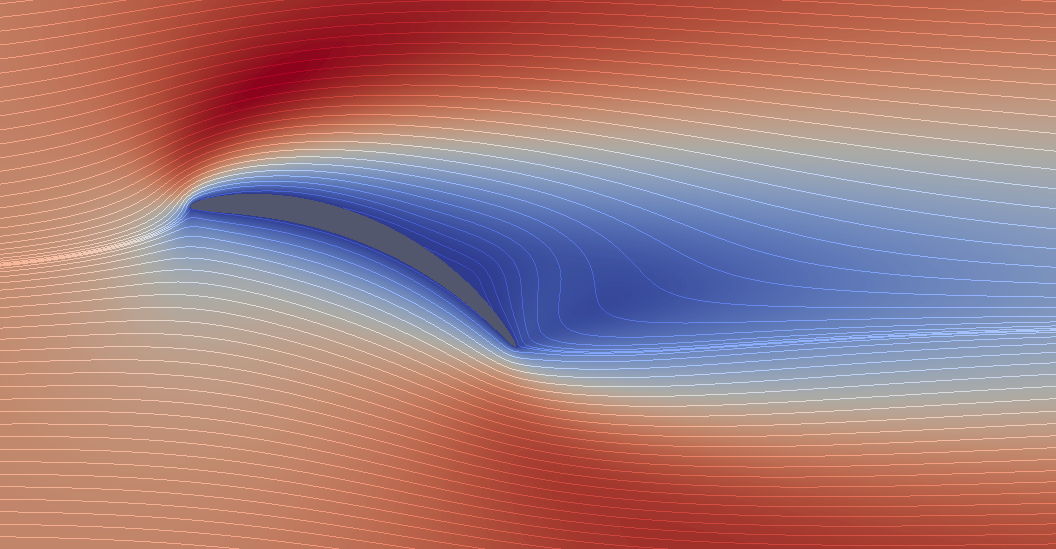
\includegraphics[width= 0.9\textwidth]{velocity_joukow}
    }
    \caption{The pressure and velocity fields of the optimal airfoil. The colour denotes the magnitude of the fields. The parameters of the airfoil are $p = (-0.0671,-0.2492,-0.4081)$.}
    \label{fig_opt_joukow}
\end{figure}

\subsection{Stability of the flow}
At larger Reynolds numbers the flow becomes unstable. The eigenvalues of the flow were investigated at Reynolds number of approximately $100$. The exact parameters of the flow and the Joukowsky-like airfoil were:
\begin{equation}
\begin{cases}
v_{in} = 1.0 \\
\rho = 1.0 \\
\mu = 0.01 \\
p = (-0.09,\, -0.16,\, \alpha)
\end{cases}
\end{equation}

The eigenvalues for $\alpha = 15^\circ$ can be seen on Figure \ref{fig:eigenvalues}. There is one eigenvalue corresponding to a wake mode which has positive real part so is a growing mode. The change of the two eigenvalues which have the largest real part can be seen on Figure \ref{fig:eigenvalue_change}.
\begin{figure}[htbp]
    \centering
    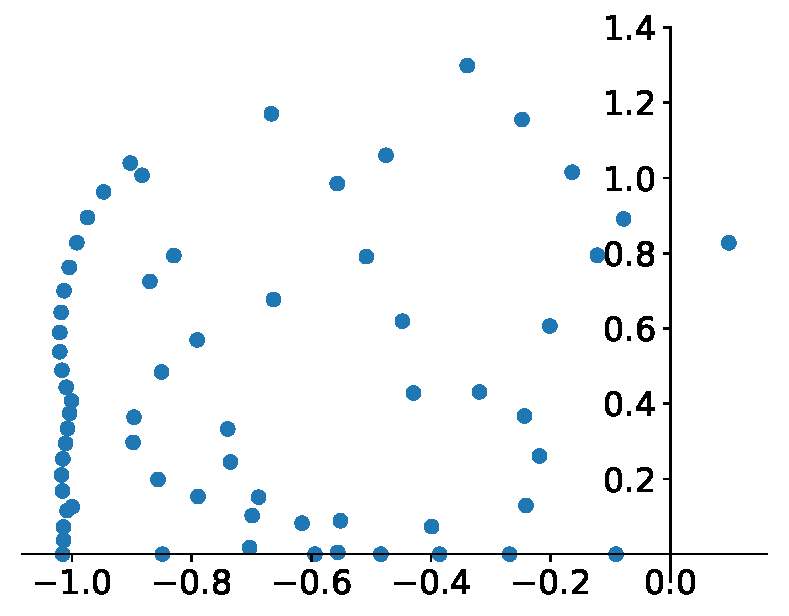
\includegraphics[width=0.7\textwidth]{sValues}
    \caption{The eigenvalues on the complex plane for $\alpha = 15^\circ$. Only the upper half plane was plotted as the eigenvalues are symmetric to the real axis. It can be seen that there is one eigenvalue of positive real part (and its pair of negative imaginary part which is not shown).}
    \label{fig:eigenvalues}
\end{figure}
\begin{figure}[htbp]
    \centering
    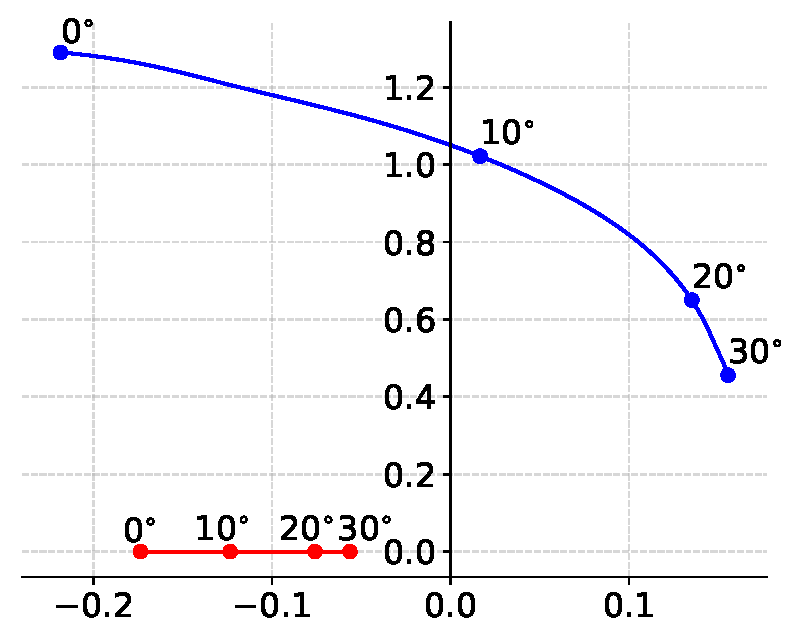
\includegraphics[width=0.7\textwidth]{maxS}
    \caption{The two important eigenvalues on the complex plane between $\alpha = 0^\circ$ and $30^\circ$.}
    \label{fig:eigenvalue_change}
\end{figure}

\subsection{Optimisation with constraint}
It is beneficial to keep the flow stable so to optimise while keeping the growth rate of the most unstable eigenmode constant and negative or zero. The area was also kept constant and the airfoil was optimised for maximum Lift-Drag ratio (without the previous repulsive term). As the Reynolds number was not too large the flow was stable when the airfoil was optimised for maximum Lift-Drag ratio with the area constraint only. To be able to test the method the real part of the most unstable eigenvalue was fixed to $-0.1$. This is a somewhat arbitrary value though. 


\section{Conclusions}
        % Summary
        \subsection{Summary}
            In this research project the adjoint method was used for shape optimisation of airfoils. The flow was validated on a circular obstacle and an ellipse was also investigated as well as the stability of the flow around an airfoil. A Joukowsky-like airfoil was optimised for maximum Lift-Drag ratio first without constraint but an additional term had to be introduced to the cost function to prevent the airfoil from overlapping (from looking like an $\infty$ sign). Next the the Lift-Drag ratio was maximised at larger Reynolds number with the constraints that the area is conserved and that the flow is kept stable enough.
            
        % Why is it useful?
        \subsection{Potential usage}
            Most importantly the derivatives of cost functions can be calculated as surface integrals after calculating the adjoint state. This means that it is not necessary to solve a differential equation for every derivative. Instead one needs to calculate the adjoint state only once (which is computationally costly) and a derivative is given by a surface integral (which is much cheaper). This can reduce the computational time dramatically especially if the airfoil is described by many parameters.
            
            The method can be used to optimise other quantities. For example the drag coefficient can be minimised easily but in this case some constraint has to be introduced because an obvious solution is an infinitely small airfoil. The constraint can be the conservation of the area or simply the choice of a parametrisation which prevents this. One can also maximise the growth rate of the eigenmodes making the flow intentionally unstable to make a vortex shredder.
            
        % Possible further work
        \subsection{Possible improvements}
            In the future other airfoils can also be optimised. Using more suitable airfoils with more parameters and higher resolution (and longer computational time) the global minimum can be approached better. The newly calculated shapes can be compared to the shape found in this paper and they are expected to be similar. With differently parametrised airfoils the repulsive term can be omitted. The method also makes it possible to perform parameter free optimisation. This requires care though. The result can reach a local minimum. One also needs to ensure that the airfoil is kept smooth.
            
\section*{Acknowledgements}

\appendix
\section*{Appendix}
\section{Derivative of the force} \label{app:force}
If the cost function ($\mathcal{J}$) is the force on the airfoil
\begin{equation}
\mathcal{J} = \int\limits_{\Omega}{{p\, \mathbf{a \cdot} \boldsymbol{\nabla} \phi} -
    {\mu \boldsymbol{\nabla}(\mathbf{a \cdot u}) \mathbf{\cdot} \boldsymbol{\nabla} \phi} - 
    {\mu a_i \frac{\partial u_j}{\partial x_i} \frac{\partial \phi}{\partial x_j}} - 
    {\rho \phi \, \mathbf{u \cdot} \boldsymbol{\nabla}(\mathbf{a \cdot u})}
    \,  \mathrm{d}x}
\end{equation}
then its derivative is given by
\begin{equation} \label{cost_change_1}
\begin{split}
d \mathcal{J} =& \int\limits_{\partial \Omega}(\mathbf{V \cdot n}) \, \bigg{(} 
{p\, \mathbf{a \cdot} \boldsymbol{\nabla} \phi} -
{\mu \boldsymbol{\nabla}(\mathbf{a \cdot u}) \cdot \boldsymbol{\nabla} \phi} \\
& \phantom{\int\limits_{\partial \Omega}(\mathbf{V \cdot n}) \, \bigg{(} \ } 
- {\mu a_i \frac{\partial u_j}{\partial x_i} \frac{\partial \phi}{\partial x_j}} - 
{\rho \phi \, \mathbf{u \cdot} \boldsymbol{\nabla}(\mathbf{a \cdot u})} 
\bigg{)} \, \mathrm{d}s \ + \\
&\int\limits_{\Omega} {p' \mathbf{a \cdot} \boldsymbol{\nabla} \phi} - 
{\mu \boldsymbol{\nabla}(\mathbf{a \cdot u'}) \cdot \boldsymbol{\nabla} \phi} -
{\mu a_i \frac{\partial u'_j}{\partial x_i} \frac{\partial \phi}{\partial x_j}} \\ 
& \phantom{\int\limits_{\Omega} \ }
- {\rho \phi \, \mathbf{u' \cdot} \boldsymbol{\nabla}(\mathbf{a \cdot u})} - 
{\rho \phi \, \mathbf{u \cdot} \boldsymbol{\nabla}(\mathbf{a \cdot u'})}
\,  \mathrm{d}x \ + \\
&\int\limits_{\Omega} p\, \mathbf{a \cdot} \boldsymbol{\nabla} \phi' -
{\mu \boldsymbol{\nabla}(\mathbf{a \cdot u}) \cdot \boldsymbol{\nabla} \phi'} - 
{\mu a_i \frac{\partial u_j}{\partial x_i} \frac{\partial \phi'}{\partial x_j}} - 
{\rho \phi' \, \mathbf{u \cdot} \boldsymbol{\nabla}(\mathbf{a \cdot u})}
\, \mathrm{d}x
\end{split}
\end{equation}
where $\mathbf{V}$ is the domain deformation vector.

If we examine the above equation term by term we get for the first term in $d \mathcal{J}$:
\begin{equation} \label{cost_change_term_1}
\int\limits_{\Gamma_0}{(\mathbf{V \cdot n}) \, \bigg{(} 
    {p\, \mathbf{a \cdot} \boldsymbol{\nabla} \phi} -
    {\mu \boldsymbol{\nabla}(\mathbf{a \cdot u}) \cdot \boldsymbol{\nabla} \phi} - 
    {\mu a_i \frac{\partial u_j}{\partial x_i} \frac{\partial \phi}{\partial x_j}} 
    \bigg{)}} \, \mathrm{d}s
\end{equation}
because $\mathbf{V}$ is zero on the outer boundaries as we are deforming only the airfoil and $\mathbf{u}$ is zero on the airfoil boundary.

If we integrate by parts the second term in $d \mathcal{J}$ we get:
\begin{equation}
\begin{split}
&\int\limits_{\Omega}{p' \mathbf{a \cdot} \boldsymbol{\nabla} \phi} \, \mathrm{d}x \ + \\
&\int\limits_{\Omega}u'_i \bigg{(}
{\mu a_i \nabla^2 \phi} + 
{\mu a_j \frac{\partial^2 \phi}{\partial x_i \partial x_j}}  - 
{\rho \phi \frac{\partial (\mathbf{a \cdot u})}{\partial x_i}} + 
{\rho a_i \frac{\partial (\phi u_j)}{\partial x_j}}
\bigg{)}\, \mathrm{d}x \ + \\
&\int\limits_{\partial \Omega}{-\mu (\mathbf{a \cdot u'}) (\boldsymbol{\nabla} \phi \mathbf{\cdot n})} - 
{\mu (\mathbf{u' \cdot} \boldsymbol{\nabla} \phi) (\mathbf{a \cdot n})} - 
{\rho \phi (\mathbf{a \cdot u'}) (\mathbf{u \cdot n})}
\, \mathrm{d}s
\end{split}
\end{equation}
The first term in the second line vanishes because of the definition of $\phi$ (equation \ref{phi_definition}). The last term in the third line vanishes as well because on a boundary either $\phi$ or $\mathbf{u}$ is zero. If we expand the last term in the second line one term vanishes because $\mathbf{u}$ is divergence free (equation \ref{NS_2}). Then the second term in $d \mathcal{J}$ becomes:
\begin{equation} \label{cost_change_term_2}
\begin{split}
&\int\limits_{\Omega}{p' \mathbf{a \cdot} \boldsymbol{\nabla} \phi} \, \mathrm{d}x \ + \\
&\int\limits_{\Omega}u'_i \bigg{(}
{\mu a_j \frac{\partial^2 \phi}{\partial x_i \partial x_j}}  - 
{\rho \phi \frac{\partial (\mathbf{a \cdot u})}{\partial x_i}} +
{\rho a_i (\mathbf{u \cdot} \boldsymbol{\nabla} \phi)}
\bigg{)}\, \mathrm{d}x \ + \\
&\int\limits_{\partial \Omega}{-\mu (\mathbf{a \cdot u'}) (\boldsymbol{\nabla} \phi \mathbf{\cdot n})} - 
{\mu (\mathbf{u' \cdot} \boldsymbol{\nabla} \phi) (\mathbf{a \cdot n})}
\, \mathrm{d}s
\end{split}
\end{equation}

If we integrate by parts the third term in $d \mathcal{J}$ we get:
\begin{equation}
\begin{split}
&\int\limits_{\Omega}{- \phi' (\mathbf{a \cdot} \boldsymbol{\nabla} p)} + 
{\mu \phi' \mathbf{a \cdot} \nabla^2 \mathbf{u}} + 
{\mu \phi' a_i \frac{\partial}{\partial x_i} \frac{\partial u_j}{\partial x_j}} - 
{\rho \phi' \mathbf{u \cdot} \boldsymbol{\nabla}(\mathbf{a \cdot u})}
\, \mathrm{d}x \ + \\
&\int\limits_{\partial \Omega}{p \phi' \mathbf{a \cdot n}} - 
{\mu \phi' \boldsymbol{\nabla}(\mathbf{a \cdot u}) \mathbf{\cdot n}} - 
{\mu \phi' a_i \frac{\partial u_j}{\partial x_i} n_j}
\, \mathrm{d}s
\end{split}
\end{equation}
The second line is zero because of the Navier-Stokes equations (equations \ref{NS_1} and \ref{NS_2}). Therefore the third term in $d \mathcal{J}$ is:
\begin{equation} \label{cost_change_term_3}
\int\limits_{\partial \Omega}{p \phi' \mathbf{a \cdot n}} - 
{\mu \phi' \boldsymbol{\nabla}(\mathbf{a \cdot u}) \mathbf{\cdot n}} - 
{\mu \phi' a_i \frac{\partial u_j}{\partial x_i} n_j}
\, \mathrm{d}s
\end{equation}

Introduce the adjoint state $(\mathbf{w}, r)$. The following integrals are zero for any $(\mathbf{w}, r)$ since $(\mathbf{u'}, p')$ satisfies its state equations.
\begin{equation} \label{adj_velocity_original}
0 = \int\limits_{\Omega}\mathbf{w \cdot} \bigg{(}
{\rho (\mathbf{u' \cdot} \boldsymbol{\nabla}) \mathbf{u}} + 
{\rho (\mathbf{u \cdot} \boldsymbol{\nabla}) \mathbf{u'}} + 
{\boldsymbol{\nabla} p'} - 
{\mu \nabla^2 \mathbf{u'}}
\bigg{)} \, \mathrm{d}x
\end{equation}
\begin{equation} \label{adj_pressure_original}
0 = \int\limits_{\Omega}{r \, \boldsymbol{\nabla} \mathbf{\cdot u'}} \, \mathrm{d}x
\end{equation}

If we integrate equation \ref{adj_velocity_original} by parts we get:
\begin{equation}
\begin{split}
0 = &\int\limits_{\Omega}
-p' \, \boldsymbol{\nabla} \mathbf{\cdot w}
\, \mathrm{d}x \ + \\
&\int\limits_{\Omega} u'_i \bigg{(}
\rho w_j \frac{\partial u_j}{\partial x_i} - 
\rho \frac{\partial (w_i u_j)}{\partial x_j} - 
\mu \nabla^2 w_i
\bigg{)} \, \mathrm{d}x \ + \\
&\int\limits_{\partial \Omega}
p' \, \mathbf{w \cdot n} + 
\rho (\mathbf{w \cdot u'}) (\mathbf{u \cdot n}) + 
\mu \mathbf{u' \cdot} \frac{\partial \mathbf{w}}{\partial n} - 
\mu \mathbf{w \cdot} \frac{\partial \mathbf{u'}}{\partial n}
\, \mathrm{d}s
\end{split}
\end{equation}
If we expand the second term in the second line one of the terms is zero because $\mathbf{u}$ is divergence free (equation \ref{NS_2}) and we get:
\begin{equation} \label{adj_velocity_parts}
\begin{split}
0 = &\int\limits_{\Omega}
-p' \, \boldsymbol{\nabla} \mathbf{\cdot w}
\, \mathrm{d}x \ + \\
&\int\limits_{\Omega} u'_i \bigg{(}
\rho w_j \frac{\partial u_j}{\partial x_i} - 
\rho \frac{\partial w_i}{\partial x_j} u_j - 
\mu \nabla^2 w_i
\bigg{)} \, \mathrm{d}x \ + \\
&\int\limits_{\partial \Omega}
p' \, \mathbf{w \cdot n} + 
\rho (\mathbf{w \cdot u'}) (\mathbf{u \cdot n}) + 
\mu \mathbf{u' \cdot} \frac{\partial \mathbf{w}}{\partial n} - 
\mu \mathbf{w \cdot} \frac{\partial \mathbf{u'}}{\partial n}
\, \mathrm{d}s
\end{split}
\end{equation}

If we integrate equation \ref{adj_pressure_original} by parts we get:
\begin{equation} \label{adj_pressure_parts}
\begin{split}
0 = &\int\limits_{\Omega}
- u'_i \frac{\partial r}{\partial x_i}
\, \mathrm{d}x \ + \\
&\int\limits_{\partial \Omega}
r \, (\mathbf{u' \cdot n})
\, \mathrm{d}s
\end{split}
\end{equation}

If we add together the second and third terms in $d \mathcal{J}$ (equations \ref{cost_change_term_2} and \ref{cost_change_term_3}) and the equations of the adjoint state which are zero (equations \ref{adj_velocity_parts} and \ref{adj_pressure_parts}) we get:
\begin{equation} \label{cost_change_term_2345}
\begin{split}
&\int\limits_{\Omega} p' \big{(}
\mathbf{a \cdot} \boldsymbol{\nabla} \phi -
\, \boldsymbol{\nabla} \mathbf{\cdot w}
\big{)} \, \mathrm{d}x \ + \\
&\int\limits_{\Omega} u'_i \bigg{(}
\mu a_j \frac{\partial^2 \phi}{\partial x_i \partial x_j}  - 
\rho \phi \frac{\partial (\mathbf{a \cdot u})}{\partial x_i} +
\rho a_i (\mathbf{u \cdot} \boldsymbol{\nabla} \phi) + \\
& \phantom{\int\limits_{\Omega} u'_i \bigg{(} \ }
\rho w_j \frac{\partial u_j}{\partial x_i} - 
\rho \frac{\partial w_i}{\partial x_j} u_j - 
\mu \nabla^2 w_i - 
\frac{\partial r}{\partial x_i}
\bigg{)} \, \mathrm{d}x \ + \\
&\int\limits_{\partial \Omega}
-\mu (\mathbf{a \cdot u'}) (\boldsymbol{\nabla} \phi \mathbf{\cdot n}) - 
\mu (\mathbf{u' \cdot} \boldsymbol{\nabla} \phi) (\mathbf{a \cdot n}) - 
\mu \phi' \boldsymbol{\nabla}(\mathbf{a \cdot u}) \mathbf{\cdot n} - 
\mu \phi' a_i \frac{\partial u_j}{\partial x_i} n_j
\, \mathrm{d}s \ + \\
&\int\limits_{\partial \Omega}
p \phi' \mathbf{a \cdot n} +
p' \, \mathbf{w \cdot n} + 
\rho (\mathbf{w \cdot u'}) (\mathbf{u \cdot n}) + 
\mu \mathbf{u' \cdot} \frac{\partial \mathbf{w}}{\partial n} - 
\mu \mathbf{w \cdot} \frac{\partial \mathbf{u'}}{\partial n} + 
r \, (\mathbf{u' \cdot n})
\, \mathrm{d}s
\end{split}
\end{equation}
The volume integrals vanish if we choose the adjoint state such that the terms in the brackets are zero. These give the state equations for the adjoint state $(\mathbf{w}, r)$.
\begin{equation}
\begin{split}
0 = & -\rho w_j \frac{\partial u_j}{\partial x_i} +
\rho (\mathbf{u \cdot} \boldsymbol{\nabla}) w_i +
\mu \nabla^2 w_i +
\frac{\partial r}{\partial x_i} \\ 
& -\mu \frac{\partial (\mathbf{a \cdot} \boldsymbol{\nabla} \phi)}{\partial x_i} +
\rho \phi \frac{\partial (\mathbf{a \cdot u})}{\partial x_i} - 
\rho a_i (\mathbf{u \cdot} \boldsymbol{\nabla} \phi)
\end{split}
\end{equation}
\begin{equation}
0 = \boldsymbol{\nabla} \mathbf{\cdot w} - 
\mathbf{a \cdot} \boldsymbol{\nabla} \phi
\end{equation}

The boundary conditions for the adjoint state $(\mathbf{w}, r)$ are given by the condition that the boundary integral should vanish on the outer boundaries and it should contain only $\mathbf{u'}$ only on the inside boundary but not its derivatives or $p'$. The boundary conditions for $(\mathbf{w}, r)$ will be:
\begin{equation}
\begin{cases}
\mathbf{w} = 0	 	&	\text{on}\ \Gamma_+ \\
\frac{\partial w_x}{\partial n} - a_x (\boldsymbol{\nabla} \phi \mathbf{\cdot n}) - 
\frac{\partial \phi}{\partial x} (\mathbf{a \cdot n}) = 0	&	\text{on}\ \Gamma_w \\
w_y = 0				&	\text{on}\ \Gamma_w \\
r \, \mathbf{n} + \mu \frac{\partial \mathbf{w}}{\partial n} + \rho \, \mathbf{w} (\mathbf{u \cdot n}) - 
\mu \, \mathbf{a} (\boldsymbol{\nabla} \phi \mathbf{\cdot n}) - 
\mu \boldsymbol{\nabla} \phi (\mathbf{a \cdot n}) = 0	   	&	\text{on}\ \Gamma_- \\
\mathbf{w} = 0	 	&	\text{on}\ \Gamma_0
\end{cases}
\end{equation}

Then the second and third terms in $d \mathcal{J}$ combined with the terms with the adjoint state become:
\begin{equation} \label{cost_change_term_2345_boundary}
\begin{split}
\int\limits_{\Gamma_0} (\mathbf{V \cdot n}) \bigg{(} &
\mu \mathbf{a \cdot} \frac{\partial \mathbf{u}}{\partial n} \frac{\partial \phi}{\partial n} + 
\mu \big{(} \frac{\partial \mathbf{u}}{\partial n} \mathbf{\cdot} \boldsymbol{\nabla} \phi \big{)} 
(\mathbf{a \cdot n}) - 
p \frac{\partial \phi}{\partial n} (\mathbf{a \cdot n}) + \\
&\mu \frac{\partial \phi}{\partial n} \boldsymbol{\nabla} (\mathbf{a \cdot u}) \mathbf{\cdot n} + 
\mu \frac{\partial \phi}{\partial n} a_i \frac{\partial u_j}{\partial x_i} n_j - 
\mu \frac{\partial \mathbf{u}}{\partial n} \frac{\partial \mathbf{w}}{\partial n} - 
r \frac{\partial \mathbf{u}}{\partial n} \mathbf{\cdot n}
\bigg{)} \, \mathrm{d}s
\end{split}
\end{equation}
where the boundary conditions for $(\mathbf{u'},p')$ and $\phi'$ were used (equations \ref{flow_der_boundary_conditions} \ref{phi_der_boundary_conditons}).
On $\Gamma_0$ both $\mathbf{u}$ and $\phi$ have Dirichlet boundary conditions of constant values and this means that their directional derivatives in a direction parallel to the surface is zero. Using this we can simplify some terms in the previous expression.
\begin{equation*}
\mu \mathbf{a \cdot} \frac{\partial \mathbf{u}}{\partial n} \frac{\partial \phi}{\partial n} = 
\mu \boldsymbol{\nabla}(\mathbf{a \cdot u}) \mathbf{\cdot} \boldsymbol{\nabla} \phi
\qquad \text{on} \ \Gamma_0
\end{equation*}
and
\begin{equation*}
\mu \big{(} \frac{\partial \mathbf{u}}{\partial n} \mathbf{\cdot} \boldsymbol{\nabla} \phi \big{)} 
(\mathbf{a \cdot n}) = 0
\qquad \text{on} \ \Gamma_0
\end{equation*}
because $\mathbf{u}$ is divergence free (equation \ref{NS_2}).
\begin{equation*}
p \frac{\partial \phi}{\partial n} (\mathbf{a \cdot n}) = 
p \, \mathbf{a \cdot} \boldsymbol{\nabla} \phi
\qquad \text{on} \ \Gamma_0
\end{equation*}
and
\begin{equation*}
\mu \frac{\partial \phi}{\partial n} \boldsymbol{\nabla} (\mathbf{a \cdot u}) \mathbf{\cdot n} = 
\mu \boldsymbol{\nabla} (\mathbf{a \cdot u}) \mathbf{\cdot} \boldsymbol{\nabla} \phi
\qquad \text{on} \ \Gamma_0
\end{equation*}
and
\begin{equation*}
\mu \frac{\partial \phi}{\partial n} a_i \frac{\partial u_j}{\partial x_i} n_j = 
\mu a_i \frac{\partial u_j}{\partial x_i} \frac{\partial \phi}{\partial x_j}
\qquad \text{on} \ \Gamma_0
\end{equation*}
\begin{equation*}
\mu \frac{\partial \mathbf{u}}{\partial n} \frac{\partial \mathbf{w}}{\partial n} = 
\mu \frac{\partial u_i}{\partial x_j} \frac{\partial w_i}{\partial x_j}
\qquad \text{on} \ \Gamma_0
\end{equation*}
and
\begin{equation*}
r \frac{\partial \mathbf{u}}{\partial n} \mathbf{\cdot n} = 
0
\qquad \text{on} \ \Gamma_0
\end{equation*}
again because $\mathbf{u}$ is divergence free (equation \ref{NS_2}). Substituting these results into equation \ref{cost_change_term_2345_boundary} results in:
\begin{equation}
\int\limits_{\Gamma_0} (\mathbf{V \cdot n}) \bigg{(}
2 \mu \boldsymbol{\nabla} (\mathbf{a \cdot u}) \mathbf{\cdot} \boldsymbol{\nabla} \phi - 
p \, \mathbf{a \cdot} \boldsymbol{\nabla} \phi + 
\mu a_i \frac{\partial u_j}{\partial x_i} \frac{\partial \phi}{\partial x_j} - 
\mu \frac{\partial u_i}{\partial x_j} \frac{\partial w_i}{\partial x_j}
\bigg{)} \, \mathrm{d}s
\end{equation}
If we combine this result with the first term in $d \mathcal{J}$ (equation \ref{cost_change_term_1}) we get the cost change:
\begin{equation}
\begin{split}
d \mathcal{J} = 
\int\limits_{\Gamma_0}(\mathbf{V \cdot n}) \, \bigg{(} &
p\, \mathbf{a \cdot} \boldsymbol{\nabla} \phi -
\mu \boldsymbol{\nabla}(\mathbf{a \cdot u}) \mathbf{\cdot} \boldsymbol{\nabla} \phi - 
\mu a_i \frac{\partial u_j}{\partial x_i} \frac{\partial \phi}{\partial x_j} \ + \\
&2 \mu \boldsymbol{\nabla} (\mathbf{a \cdot u}) \mathbf{\cdot} \boldsymbol{\nabla} \phi - 
p \, \mathbf{a \cdot} \boldsymbol{\nabla} \phi + 
\mu a_i \frac{\partial u_j}{\partial x_i} \frac{\partial \phi}{\partial x_j} - 
\mu \frac{\partial u_i}{\partial x_j} \frac{\partial w_i}{\partial x_j}
\bigg{)} \, \mathrm{d}s
\end{split}
\end{equation}
Some terms cancel in this expression so the derivative of the cost function is given by:
\begin{equation}
\begin{split}
d \mathcal{J} = \int\limits_{\Gamma_0}(\mathbf{V \cdot n}) \, \bigg{(} &
\mu \boldsymbol{\nabla}(\mathbf{a \cdot u}) \mathbf{\cdot} \boldsymbol{\nabla} \phi -
\mu \frac{\partial u_i}{\partial x_j} \frac{\partial w_i}{\partial x_j}
\bigg{)} \, \mathrm{d}s
\end{split}
\end{equation}

\section{Derivative of the eigenvalue} \label{app:eigenvalue}
The cost function to be investigated is the eigenvalue of some specific perturbation state.
\begin{equation}
\mathcal{J} = s
\end{equation}

The derivative of the cost function is:
\begin{equation}
d \mathcal{J} = s'
\end{equation}
Using the state equations for the change in the base flow and the perturbation field (equations \ref{NS_der_1}, \ref{NS_der_2}, \ref{perturbation_change_1}, \ref{perturbation_change_2}) for any adjoint base flow $(\mathbf{u^{\dagger}},p^{\dagger})$ and adjoint perturbation field $(\mathbf{w^{\dagger}},r^{\dagger})$ the change in the cost function can be written as:
\begin{equation}
\begin{split}
d \mathcal{J} =& \ s' \, + \\
& \int\limits_{\Omega} \mathbf{u^{\dagger *} \cdot} \bigg( 
\rho \, (\mathbf{u \cdot} \boldsymbol{\nabla}) \mathbf{u'} + 
\rho \, (\mathbf{u' \cdot} \boldsymbol{\nabla}) \mathbf{u} + 
\boldsymbol{\nabla} p' - 
\mu \, \nabla^2 \mathbf{u'}
\bigg) \, \mathrm{d} x \ + \\
& \int\limits_{\Omega} p^{\dagger *} 
\boldsymbol{\nabla} \mathbf{\cdot u'}
\, \mathrm{d} x \ + \\
& \int\limits_{\Omega} \mathbf{w^{\dagger *} \cdot} \bigg( 
\rho \, s' \, \mathbf{w} + 
\rho \, s \, \mathbf{w'} + 
\rho \, (\mathbf{w \cdot} \boldsymbol{\nabla}) \mathbf{u'} + 
\rho \, (\mathbf{w' \cdot} \boldsymbol{\nabla}) \mathbf{u} \ + \\
&\phantom{\int\limits_{\Omega} \mathbf{w^{\dagger *} \cdot} \bigg( \ }
\rho \, (\mathbf{u' \cdot} \boldsymbol{\nabla}) \mathbf{w} + 
\rho \, (\mathbf{u \cdot} \boldsymbol{\nabla}) \mathbf{w'} +
\boldsymbol{\nabla} r' - 
\mu \, \nabla^2 \mathbf{w'}
\bigg) \, \mathrm{d} x \ + \\
& \int\limits_{\Omega} r^{\dagger *} 
\boldsymbol{\nabla} \mathbf{\cdot w'}
\, \mathrm{d} x
\end{split}
\end{equation}
where asterisk denotes complex conjugation.

If we integrate the integral terms in the derivative of the cost change we get for the first row:
\begin{equation}
\begin{split}
&\int\limits_{\Omega} u'_i \bigg( 
-\rho \, \mathbf{u \cdot} \boldsymbol{\nabla} u^{\dagger *}_i + 
\rho \, \mathbf{u^{\dagger *} \cdot} \frac{\partial \mathbf{u}}{\partial x_i} - 
\mu \, \nabla^2 u^{\dagger *}_i
\bigg) \, \mathrm{d} x \ + \\
&\int\limits_{\Omega} 
- p' \, \boldsymbol{\nabla} \mathbf{\cdot u^{\dagger *}}
\, \mathrm{d} x \ + \\
&\int\limits_{\partial \Omega}
\rho \, (\mathbf{u^{\dagger *} \cdot u'}) (\mathbf{u \cdot n}) + 
p' \, (\mathbf{u^{\dagger *} \cdot n}) + 
\mu \, \mathbf{u' \cdot} \frac{\partial \mathbf{u^{\dagger *}}}{\partial n} - 
\mu \, \mathbf{u^{\dagger *} \cdot} \frac{\partial \mathbf{u'}}{\partial n}
\, \mathrm{d} s
\end{split}
\end{equation}
where it was used that $\mathbf{u}$ is divergence free (equation \ref{NS_2}).

The second line in $d \mathcal{J}$ becomes:
\begin{equation}
\begin{split}
&\int\limits_{\Omega}
- u'_i \, \frac{\partial p^{\dagger *}}{\partial x_i}
\, \mathrm{d} x \ + \\
&\int\limits_{\partial \Omega}
p^{\dagger *} (\mathbf{u' \cdot n})
\, \mathrm{d} s
\end{split}
\end{equation}

The third line in $d \mathcal{J}$ becomes:
\begin{equation}
\begin{split}
&\int\limits_{\Omega}
\rho \, s' (\mathbf{w^{\dagger *} \cdot w})
\, \mathrm{d} x \ + \\
&\int\limits_{\Omega} u'_i \bigg( 
\rho \, \mathbf{w^{\dagger *} \cdot} \frac{\partial \mathbf{w}}{\partial x_i} - 
\rho \, (\mathbf{w \cdot} \boldsymbol{\nabla}) w^{\dagger *}_i
\bigg) \, \mathrm{d} x \ + \\
&\int\limits_{\Omega} w'_i \bigg( 
\rho \, s \, w^{\dagger *}_i + 
\rho \, \mathbf{w^{\dagger *} \cdot} \frac{\partial \mathbf{u}}{\partial x_i} - 
\rho \, (\mathbf{u \cdot} \boldsymbol{\nabla}) w^{\dagger *}_i - 
\mu \, \nabla^2 w^{\dagger *}_i
\bigg) \, \mathrm{d} x \ + \\
&\int\limits_{\Omega}
- r' \, \boldsymbol{\nabla} \mathbf{\cdot w^{\dagger *}}
\, \mathrm{d} x \ + \\
&\int\limits_{\partial \Omega}
\rho \, (\mathbf{u' \cdot w^{\dagger *}}) (\mathbf{w \cdot n}) + 
\rho \, (\mathbf{w^{\dagger *} \cdot w'}) (\mathbf{u \cdot n}) + 
r' \, (\mathbf{w^{\dagger *} \cdot n}) \ + \\
& \phantom{\int\limits_{\partial \Omega} \ }
\mu \, \mathbf{w' \cdot} \frac{\partial \mathbf{w^{\dagger *}}}{\partial n} - 
\mu \, \mathbf{w^{\dagger *} \cdot} \frac{\partial \mathbf{w'}}{\partial n}
\, \mathrm{d} s
\end{split}
\end{equation}
where again it was used that both $\mathbf{u}$ and $\mathbf{w}$ are divergence free (equations \ref{NS_2} and \ref{perturbation_2}).

The fourth line in $d \mathcal{J}$ becomes:
\begin{equation}
\begin{split}
&\int\limits_{\Omega}
- w'_i \, \frac{\partial r^{\dagger *}}{\partial x_i}
\, \mathrm{d} x \ + \\
&\int\limits_{\partial \Omega}
r^{\dagger *} \, (\mathbf{w' \cdot n})
\, \mathrm{d} s
\end{split}
\end{equation}

Combining the results above gives the expression for the derivative of the cost function:
\begin{equation}
\begin{split}
d \mathcal{J} = \ &
s' \left( 1 + 
\int\limits_{\Omega} \rho \, (\mathbf{w^{\dagger *} \cdot w}) 
\, \mathrm{d} x
\right) \ + \\
&\int\limits_{\Omega}
-p' \, \boldsymbol{\nabla} \mathbf{\cdot u^{\dagger *}}
\, \mathrm{d} x \ + \\
&\int\limits_{\Omega} u'_i \bigg( 
- \rho (\mathbf{u \cdot} \boldsymbol{\nabla}) u^{\dagger*}_i + 
\rho \mathbf{u^{\dagger*} \cdot} \frac{\partial \mathbf{u}}{\partial x_i} - 
\mu \, \nabla^2 u^{\dagger*}_i \\ 
& \phantom{\int\limits_{\Omega} u'_i \bigg( \ }
- \frac{\partial p^{\dagger*}}{\partial x_i} + 
\rho \, \mathbf{w^{\dagger*} \cdot} \frac{\partial \mathbf{w}}{\partial x_i} - 
\rho \, (\mathbf{w \cdot} \boldsymbol{\nabla}) w^{\dagger*}_i
\bigg) \, \mathrm{d} x \ + \\
&\int\limits_{\Omega}
-r' \, \boldsymbol{\nabla} \mathbf{\cdot w^{\dagger *}}
\, \mathrm{d} x \ + \\
&\int\limits_{\Omega} w'_i \bigg( 
\rho \, s \, w^{\dagger*}_i + 
\rho \mathbf{w^{\dagger*} \cdot} \frac{\partial \mathbf{u}}{\partial x_i} - 
\rho \, (\mathbf{u \cdot} \boldsymbol{\nabla}) w^{\dagger*}_i - 
\mu \, \nabla^2 w^{\dagger*}_i - 
\frac{\partial r^{\dagger*}}{\partial x_i}
\bigg) \, \mathrm{d} x \ + \\
&\int\limits_{\partial \Omega}
\rho \, (\mathbf{u^{\dagger*} \cdot u'}) (\mathbf{u \cdot n}) + 
p' \, (\mathbf{u^{\dagger} \cdot n}) + 
\mu, \mathbf{u' \cdot} \frac{\partial \mathbf{u^{\dagger*}}}{\partial n} - 
\mu \, \mathbf{u^{\dagger*} \cdot} \frac{\partial \mathbf{u'}}{\partial n} \ + \\
&\phantom{\int\limits_{\partial \Omega} \ }
p^{\dagger*} \, (\mathbf{u' \cdot n}) + 
\rho \, (\mathbf{u' \cdot w^{\dagger*}}) (\mathbf{w \cdot n}) + 
\rho \, (\mathbf{w^{\dagger*} \cdot w'}) (\mathbf{u \cdot n}) \ + \\
&\phantom{\int\limits_{\partial \Omega} \ }
r' \, (\mathbf{w^{\dagger*} \cdot n}) + 
\mu \, \mathbf{w' \cdot} \frac{\partial \mathbf{w^{\dagger*}}}{\partial n} - 
\mu \, \mathbf{w^{\dagger*} \cdot} \frac{\partial \mathbf{w'}}{\partial n} + 
r^{\dagger*} \, (\mathbf{w' \cdot n})
\, \mathrm{d} s
\end{split}
\end{equation}

The volume integrals should vanish as well as the boundary term on the outer boundaries and the terms containing the derivatives of $(\mathbf{u'}, p')$ or the derivatives of $(\mathbf{w'}, r')$ on the airfoil boundary. This along with the boundary contitions of $(\mathbf{u'}, p')$ and $(\mathbf{w'}, r')$ (equations \ref{flow_der_boundary_conditions} and \ref{perturbation_change_bcs}) gives the state equations or the adjoint states and their boundary conditions.

The equations for the adjoint perturbation's complex conjugate $(\mathbf{w^{\dagger*}}, r^{\dagger*})$:
\begin{equation}
\rho \, \mathbf{w^{\dagger*} \cdot} \frac{\partial \mathbf{u}}{\partial x_i} - 
\rho \, (\mathbf{u \cdot} \boldsymbol{\nabla}) w^{\dagger*}_i - 
\mu \, \nabla^2 w^{\dagger*}_i - 
\frac{\partial r^{\dagger*}}{\partial x_i} = 
-\rho \, s \, w^{\dagger*}_i
\end{equation}
\begin{equation}
\boldsymbol{\nabla} \mathbf{\cdot w^{\dagger*}} = 0
\end{equation}
with boundary conditions:
\begin{equation}
\begin{cases}
\mathbf{w^{\dagger*}} = 0 & \text{on } \Gamma_+ \\
\frac{\partial w^{\dagger*}_x}{\partial n} = 0 & \text{on } \Gamma_w \\
w^{\dagger*}_y = 0 & \text{on } \Gamma_w \\
\rho \, \mathbf{w^{\dagger*}} (\mathbf{u \cdot n}) + \mu \, \frac{\partial \mathbf{w^{\dagger*}}}{\partial n} + 
r^{\dagger*} \, \mathbf{n} = 0 & \text{on } \Gamma_- \\
\mathbf{w^{\dagger*}} = 0 & \text{on } \Gamma_0
\end{cases}
\end{equation}
Since these equations are homogenious and linear in $(\mathbf{w^{\dagger*}}, r^{\dagger*})$ the zero state is a solution. To find the real solution one needs to find solutions of the eigenvalue equation (as if $s$ were free to vary) and choose the solution where the eigenvalue is closest to the actual value of $s$. The difference between the two eigenvalues should be due to computational errors.

The perturbation state $(\mathbf{w}, r)$ can be normalised using the constraint:
\begin{equation}
0 = 1 + \int\limits_{\Omega}
\rho \, (\mathbf{w^{\dagger*} \cdot w})
\, \mathrm{d} x
\end{equation}

The equations of the adjoint base flow's complex conjugate $(\mathbf{u^{\dagger*}}, p^{\dagger*})$ are:
\begin{equation}
0 = - \rho \, (\mathbf{u \cdot} \boldsymbol{\nabla}) u^{\dagger*}_i + 
\rho \, \mathbf{u^{\dagger*} \cdot} \frac{\partial \mathbf{u}}{\partial x_i} - 
\mu \, \nabla^2 u^{\dagger*}_i - 
\frac{p^{\dagger*}}{\partial x_i} + 
\rho \, \mathbf{w^{\dagger*} \cdot} \frac{\partial \mathbf{w}}{\partial x_i} - 
\rho \, (\mathbf{w \cdot} \boldsymbol{\nabla}) w^{\dagger*}_i
\end{equation}
\begin{equation}
0 = \boldsymbol{\nabla} \mathbf{\cdot u^{\dagger*}}
\end{equation}
with boundary conditions
\begin{equation}
\begin{cases}
\mathbf{u^{\dagger*}} = 0 & \text{on } \Gamma_+ \\
\frac{\partial u^{\dagger*}_x}{\partial n} = 0 & \text{on } \Gamma_w \\
u^{\dagger*}_y = 0 & \text{on } \Gamma_w \\
\rho \, \mathbf{u^{\dagger*}} (\mathbf{u \cdot n}) + \mu \, \frac{\partial \mathbf{u^{\dagger*}}}{\partial n} + 
p^{\dagger*} \, \mathbf{n} + \rho \, \mathbf{w^{\dagger*}} (\mathbf{w \cdot n}) = 0 & \text{on } \Gamma_- \\
\mathbf{u^{\dagger*}} = 0 & \text{on } \Gamma_0
\end{cases}
\end{equation}

Using these adjoint states the derivative of the cost function (the derivative of the eigenvalue) becomes:
\begin{equation}
d \mathcal{J} = \int\limits_{\Gamma_0} (\mathbf{V \cdot n}) \left( 
-mu \, \frac{\partial \mathbf{u}}{\partial n} \frac{\partial \mathbf{u^{\dagger*}}}{\partial n} - 
p^{\dagger*} \frac{\partial \mathbf{u}}{\partial n} \mathbf{\cdot n} - 
\mu \, \frac{\partial \mathbf{w}}{\partial n} \frac{\partial \mathbf{w^{\dagger*}}}{\partial n} - 
r^{\dagger*} \frac{\partial \mathbf{w}}{\partial n} \mathbf{\cdot n}
\right) \mathrm{d} s
\end{equation}
The terms in the brackets can be simplified.

\begin{equation*}
\frac{\partial \mathbf{u}}{\partial n} \frac{\partial \mathbf{u^{\dagger*}}}{\partial n} = 
\frac{\partial u_i}{\partial x_j} \frac{\partial u^{\dagger*}_i}{\partial x_j}
\quad \text{on } \Gamma_0
\end{equation*}
because of the Dirichlet boundary conditions of constant value of $\mathbf{u}$ and $\mathbf{u^{\dagger*}}$.

\begin{equation*}
\frac{\partial \mathbf{u}}{\partial n} \mathbf{\cdot n} = 0 \quad \text{on } \Gamma_0
\end{equation*}
because of the Dirichlet boundary conditions of constant value and because $\mathbf{u}$ is divergence free (equation \ref{NS_2}).

\begin{equation*}
\frac{\partial \mathbf{w}}{\partial n} \frac{\partial \mathbf{w^{\dagger*}}}{\partial n} = 
\frac{\partial w_i}{\partial x_j} \frac{\partial w^{\dagger*}}{\partial x_j}
\quad \text{on } \Gamma_0
\end{equation*}
because of the Dirichlet boundary conditions of constant value of $\mathbf{w}$ and $\mathbf{w^{\dagger*}}$.

\begin{equation*}
\frac{\partial \mathbf{w}}{\partial n} \mathbf{\cdot n} = 0 \quad \text{on } \Gamma_0
\end{equation*}
because of the Dirichlet boundary conditions of constant value and because $\mathbf{w}$ is divergence free (equation \ref{perturbation_2}).

After simplifying the above terms the derivative of the cost function (the derivative of the eigenvalue) becomes 
\begin{equation}
d \mathcal{J} = s' = \int\limits_{\Gamma_0} - (\mathbf{V \cdot n}) \left( 
\mu \, \frac{\partial u_i}{\partial x_j} \frac{\partial u^{\dagger*}_i}{\partial x_j} + 
\mu \, \frac{\partial w_i}{\partial x_j} \frac{\partial w^{\dagger*}_i}{\partial x_j}
\right) \, \mathrm{d} s 
\end{equation}

\bibliographystyle{unsrt}
\bibliography{references}

\end{document}